\chapter{Wstęp}
Dla prostoty i przejrzystości sprawozdania wykorzystane zostały oznaczenia pierwotnie wprowadzone w skrypcie z laboratorium\@.

\chapter{Algorytm DMC}

Aby zaimplementować algorytm DMC wstępnie pobrano odpowiedź skokową regulowanego obiektu. Wykonano skok sterowania od 30\% do 50\% i wynikowy przebieg temperatury wyjściowej przedstawiono na rysunku \ref{step}.

\begin{figure}[H]
	\centering
	%err =676767.9754
\definecolor{mycolor1}{rgb}{0.00000,0.44700,0.74100}%
\definecolor{mycolor2}{rgb}{0.85000,0.32500,0.09800}%
%
\begin{tikzpicture}

\begin{axis}[%
width=5.167in,
height=0.656in,
at={(0.646in,0.525in)},
scale only axis,
xmin=0,
xmax=400,
xtick={0,50,100,150,200,250,300,350,400},
xlabel style={font=\color{white!15!black}},
xlabel={$k$},
ymin=-20,
ymax=0,
ytick={-20,-10,0},
ylabel style={font=\color{white!15!black}},
ylabel={$u$},
axis background/.style={fill=white}
]
\addplot[const plot, color=mycolor1, forget plot] table[row sep=crcr] {%
1	-20\\
2	-20\\
3	-20\\
4	-20\\
5	-20\\
6	-20\\
7	-20\\
8	-20\\
9	-20\\
10	-20\\
11	-20\\
12	-20\\
13	0\\
14	0\\
15	0\\
16	0\\
17	0\\
18	0\\
19	0\\
20	0\\
21	0\\
22	0\\
23	0\\
24	0\\
25	0\\
26	0\\
27	0\\
28	0\\
29	0\\
30	0\\
31	0\\
32	0\\
33	0\\
34	0\\
35	0\\
36	0\\
37	0\\
38	0\\
39	0\\
40	0\\
41	0\\
42	0\\
43	0\\
44	0\\
45	0\\
46	0\\
47	0\\
48	0\\
49	0\\
50	0\\
51	0\\
52	0\\
53	0\\
54	0\\
55	0\\
56	0\\
57	0\\
58	0\\
59	0\\
60	0\\
61	0\\
62	0\\
63	0\\
64	0\\
65	0\\
66	0\\
67	0\\
68	0\\
69	0\\
70	0\\
71	0\\
72	0\\
73	0\\
74	0\\
75	0\\
76	0\\
77	0\\
78	0\\
79	0\\
80	0\\
81	0\\
82	0\\
83	0\\
84	0\\
85	0\\
86	0\\
87	0\\
88	0\\
89	0\\
90	0\\
91	0\\
92	0\\
93	0\\
94	0\\
95	0\\
96	0\\
97	0\\
98	0\\
99	0\\
100	0\\
101	0\\
102	0\\
103	0\\
104	0\\
105	0\\
106	0\\
107	0\\
108	0\\
109	0\\
110	0\\
111	0\\
112	0\\
113	0\\
114	0\\
115	0\\
116	0\\
117	0\\
118	0\\
119	0\\
120	0\\
121	0\\
122	0\\
123	0\\
124	0\\
125	0\\
126	0\\
127	0\\
128	0\\
129	0\\
130	0\\
131	0\\
132	0\\
133	0\\
134	0\\
135	0\\
136	0\\
137	0\\
138	0\\
139	0\\
140	0\\
141	0\\
142	0\\
143	0\\
144	0\\
145	0\\
146	0\\
147	0\\
148	0\\
149	0\\
150	0\\
151	0\\
152	0\\
153	0\\
154	0\\
155	0\\
156	0\\
157	0\\
158	0\\
159	0\\
160	0\\
161	0\\
162	0\\
163	0\\
164	0\\
165	0\\
166	0\\
167	0\\
168	0\\
169	0\\
170	0\\
171	0\\
172	0\\
173	0\\
174	0\\
175	0\\
176	0\\
177	0\\
178	0\\
179	0\\
180	0\\
181	0\\
182	0\\
183	0\\
184	0\\
185	0\\
186	0\\
187	0\\
188	0\\
189	0\\
190	0\\
191	0\\
192	0\\
193	0\\
194	0\\
195	0\\
196	0\\
197	0\\
198	0\\
199	0\\
200	0\\
201	0\\
202	0\\
203	0\\
204	0\\
205	0\\
206	0\\
207	0\\
208	0\\
209	0\\
210	0\\
211	0\\
212	0\\
213	0\\
214	0\\
215	0\\
216	0\\
217	0\\
218	0\\
219	0\\
220	0\\
221	0\\
222	0\\
223	0\\
224	0\\
225	0\\
226	0\\
227	0\\
228	0\\
229	0\\
230	0\\
231	0\\
232	0\\
233	0\\
234	0\\
235	0\\
236	0\\
237	0\\
238	0\\
239	0\\
240	0\\
241	0\\
242	0\\
243	0\\
244	0\\
245	0\\
246	0\\
247	0\\
248	0\\
249	0\\
250	0\\
251	0\\
252	0\\
253	0\\
254	0\\
255	0\\
256	0\\
257	0\\
258	0\\
259	0\\
260	0\\
261	0\\
262	0\\
263	0\\
264	0\\
265	0\\
266	0\\
267	0\\
268	0\\
269	0\\
270	0\\
271	0\\
272	0\\
273	0\\
274	0\\
275	0\\
276	0\\
277	0\\
278	0\\
279	0\\
280	0\\
281	0\\
282	0\\
283	0\\
284	0\\
285	0\\
286	0\\
287	0\\
288	0\\
289	0\\
290	0\\
291	0\\
292	0\\
293	0\\
294	0\\
295	0\\
296	0\\
297	0\\
298	0\\
299	0\\
300	0\\
301	0\\
302	0\\
303	0\\
304	0\\
305	0\\
306	0\\
307	0\\
308	0\\
309	0\\
310	0\\
311	0\\
312	0\\
313	0\\
314	0\\
315	0\\
316	0\\
317	0\\
318	0\\
319	0\\
320	0\\
321	0\\
322	0\\
323	0\\
324	0\\
325	0\\
326	0\\
327	0\\
328	0\\
329	0\\
330	0\\
331	0\\
332	0\\
333	0\\
334	0\\
335	0\\
336	0\\
337	0\\
338	0\\
339	0\\
340	0\\
341	0\\
342	0\\
343	0\\
344	0\\
345	0\\
346	0\\
347	0\\
348	0\\
349	0\\
350	0\\
351	0\\
352	0\\
353	0\\
354	0\\
355	0\\
356	0\\
357	0\\
358	0\\
359	0\\
360	0\\
361	0\\
362	0\\
363	0\\
364	0\\
365	0\\
366	0\\
367	0\\
368	0\\
369	0\\
370	0\\
371	0\\
372	0\\
373	0\\
374	0\\
375	0\\
376	0\\
377	0\\
378	0\\
379	0\\
380	0\\
381	0\\
382	0\\
383	0\\
384	0\\
385	0\\
386	0\\
387	0\\
388	0\\
389	0\\
390	0\\
391	0\\
392	0\\
393	0\\
394	0\\
395	0\\
396	0\\
397	0\\
398	0\\
399	0\\
400	0\\
};
\end{axis}

\begin{axis}[%
width=5.167in,
height=2.625in,
at={(0.646in,1.619in)},
scale only axis,
xmin=0,
xmax=400,
xtick={0,50,100,150,200,250,300,350,400},
ymin=36,
ymax=44,
ytick={36,37,38,39,40,41,42,43,44},
yticklabels={{36},{37},{38},{39},{40},{41},{42},{43},{44}},
ylabel style={font=\color{white!15!black}},
ylabel={$y$},
axis background/.style={fill=white}
]
\addplot [color=mycolor1, forget plot]
  table[row sep=crcr]{%
1	36.37\\
2	36.37\\
3	36.37\\
4	36.37\\
5	36.37\\
6	36.37\\
7	36.37\\
8	36.37\\
9	36.37\\
10	36.37\\
11	36.37\\
12	36.37\\
13	36.37\\
14	36.37\\
15	36.37\\
16	36.37\\
17	36.37\\
18	36.37\\
19	36.37\\
20	36.37\\
21	36.37\\
22	36.43\\
23	36.43\\
24	36.43\\
25	36.43\\
26	36.43\\
27	36.43\\
28	36.43\\
29	36.5\\
30	36.5\\
31	36.56\\
32	36.56\\
33	36.62\\
34	36.68\\
35	36.68\\
36	36.75\\
37	36.81\\
38	36.87\\
39	36.93\\
40	37\\
41	37.06\\
42	37.18\\
43	37.18\\
44	37.25\\
45	37.37\\
46	37.43\\
47	37.5\\
48	37.56\\
49	37.68\\
50	37.75\\
51	37.81\\
52	37.87\\
53	37.87\\
54	38\\
55	38\\
56	38.12\\
57	38.12\\
58	38.18\\
59	38.25\\
60	38.31\\
61	38.37\\
62	38.43\\
63	38.56\\
64	38.62\\
65	38.68\\
66	38.75\\
67	38.81\\
68	38.81\\
69	38.87\\
70	38.93\\
71	38.93\\
72	39\\
73	39.06\\
74	39.12\\
75	39.18\\
76	39.25\\
77	39.31\\
78	39.37\\
79	39.43\\
80	39.5\\
81	39.56\\
82	39.62\\
83	39.68\\
84	39.68\\
85	39.68\\
86	39.75\\
87	39.81\\
88	39.81\\
89	39.87\\
90	39.87\\
91	39.87\\
92	39.93\\
93	39.93\\
94	40\\
95	40\\
96	40.06\\
97	40.12\\
98	40.12\\
99	40.12\\
100	40.18\\
101	40.25\\
102	40.31\\
103	40.31\\
104	40.37\\
105	40.43\\
106	40.43\\
107	40.43\\
108	40.5\\
109	40.5\\
110	40.5\\
111	40.56\\
112	40.56\\
113	40.56\\
114	40.62\\
115	40.68\\
116	40.68\\
117	40.68\\
118	40.68\\
119	40.75\\
120	40.75\\
121	40.75\\
122	40.75\\
123	40.81\\
124	40.81\\
125	40.81\\
126	40.87\\
127	40.87\\
128	40.87\\
129	40.93\\
130	40.93\\
131	40.93\\
132	41\\
133	41\\
134	41\\
135	41.06\\
136	41.06\\
137	41.12\\
138	41.18\\
139	41.18\\
140	41.18\\
141	41.18\\
142	41.18\\
143	41.18\\
144	41.18\\
145	41.18\\
146	41.25\\
147	41.25\\
148	41.25\\
149	41.31\\
150	41.31\\
151	41.31\\
152	41.31\\
153	41.31\\
154	41.37\\
155	41.37\\
156	41.37\\
157	41.37\\
158	41.37\\
159	41.37\\
160	41.37\\
161	41.37\\
162	41.37\\
163	41.37\\
164	41.43\\
165	41.43\\
166	41.43\\
167	41.43\\
168	41.43\\
169	41.43\\
170	41.5\\
171	41.5\\
172	41.5\\
173	41.56\\
174	41.56\\
175	41.56\\
176	41.56\\
177	41.62\\
178	41.68\\
179	41.68\\
180	41.68\\
181	41.75\\
182	41.75\\
183	41.75\\
184	41.81\\
185	41.81\\
186	41.87\\
187	41.87\\
188	41.87\\
189	41.87\\
190	41.87\\
191	41.81\\
192	41.81\\
193	41.81\\
194	41.81\\
195	41.81\\
196	41.81\\
197	41.81\\
198	41.81\\
199	41.87\\
200	41.87\\
201	41.87\\
202	41.93\\
203	41.93\\
204	41.93\\
205	41.93\\
206	41.93\\
207	41.93\\
208	41.93\\
209	41.93\\
210	41.93\\
211	41.93\\
212	41.93\\
213	41.93\\
214	41.93\\
215	41.93\\
216	42\\
217	42\\
218	42\\
219	42.06\\
220	42.06\\
221	42.06\\
222	42.12\\
223	42.12\\
224	42.12\\
225	42.12\\
226	42.18\\
227	42.12\\
228	42.12\\
229	42.12\\
230	42.12\\
231	42.06\\
232	42.06\\
233	42.06\\
234	42.06\\
235	42.06\\
236	42.06\\
237	42.12\\
238	42.12\\
239	42.12\\
240	42.18\\
241	42.18\\
242	42.25\\
243	42.31\\
244	42.31\\
245	42.31\\
246	42.31\\
247	42.37\\
248	42.31\\
249	42.31\\
250	42.31\\
251	42.31\\
252	42.31\\
253	42.31\\
254	42.31\\
255	42.37\\
256	42.37\\
257	42.37\\
258	42.37\\
259	42.43\\
260	42.43\\
261	42.43\\
262	42.43\\
263	42.43\\
264	42.43\\
265	42.43\\
266	42.43\\
267	42.43\\
268	42.43\\
269	42.43\\
270	42.43\\
271	42.43\\
272	42.43\\
273	42.43\\
274	42.43\\
275	42.43\\
276	42.43\\
277	42.43\\
278	42.5\\
279	42.5\\
280	42.5\\
281	42.5\\
282	42.5\\
283	42.5\\
284	42.5\\
285	42.5\\
286	42.5\\
287	42.5\\
288	42.5\\
289	42.5\\
290	42.5\\
291	42.5\\
292	42.56\\
293	42.5\\
294	42.5\\
295	42.5\\
296	42.5\\
297	42.5\\
298	42.5\\
299	42.5\\
300	42.43\\
301	42.43\\
302	42.43\\
303	42.43\\
304	42.43\\
305	42.43\\
306	42.43\\
307	42.43\\
308	42.5\\
309	42.5\\
310	42.5\\
311	42.56\\
312	42.56\\
313	42.62\\
314	42.68\\
315	42.75\\
316	42.81\\
317	42.81\\
318	42.81\\
319	42.87\\
320	42.87\\
321	42.93\\
322	42.93\\
323	42.93\\
324	43\\
325	43\\
326	43.06\\
327	43.06\\
328	43.06\\
329	43.06\\
330	43.06\\
331	43.12\\
332	43.12\\
333	43.12\\
334	43.12\\
335	43.12\\
336	43.12\\
337	43.12\\
338	43.12\\
339	43.12\\
340	43.12\\
341	43.12\\
342	43.12\\
343	43.12\\
344	43.12\\
345	43.12\\
346	43.12\\
347	43.12\\
348	43.12\\
349	43.12\\
350	43.12\\
351	43.12\\
352	43.12\\
353	43.12\\
354	43.12\\
355	43.06\\
356	43.06\\
357	43.06\\
358	43\\
359	43\\
360	42.93\\
361	42.93\\
362	42.93\\
363	42.93\\
364	42.93\\
365	42.93\\
366	42.93\\
367	42.93\\
368	43\\
369	43\\
370	43\\
371	43\\
372	43\\
373	43\\
374	43\\
375	43.06\\
376	43\\
377	43\\
378	43\\
379	43\\
380	43\\
381	43\\
382	43\\
383	43\\
384	43\\
385	43\\
386	43\\
387	42.93\\
388	42.93\\
389	42.93\\
390	42.93\\
391	43\\
392	42.93\\
393	42.93\\
394	42.93\\
395	42.93\\
396	42.93\\
397	42.93\\
398	42.93\\
399	42.93\\
400	42.87\\
};
\end{axis}
\end{tikzpicture}%
	\caption{Odpowiedź skokowa układu}
	\label{step}
\end{figure}

Sama implementacja algorytmu jest praktycznie identyczna jak w poprzednim laboratorium, opisywanie jej szczegółów zostanie więc pominięte. Tak jak ostatnio, niezbędne parametry do regulacji wyznaczono korzystając ze skryptu \verb|params.m| w MATLABie, po czym skopiowano je do pliku źródłowego \verb|main.c| w miejscu wykonywania głównej pętli regulacji.

Na podstawie czasu stabilizacji odpowiedzi skokowej wyznaczono wstępnie parametr $ D = 300 $, a następnie ustalono $ N $ i $ N_\mathrm{u} $ na równe $ D $ jako teoretycznie optymalne. Przy tych wstępnych parametrach przetestowano dwie różne wartości $ \lambda $ i porównano ich przebiegi (rys. \ref{DMC1} i \ref{DMC2}) ze sobą. Odpowiedź o $ \lambda $ mniejszej zdaje się być lepsza, choć możliwy jest wpływ różnych zakłóceń na uzyskane przebiegi.


\begin{figure}[ht]
\centering
%err =1352.1787
\definecolor{mycolor1}{rgb}{0.00000,0.44700,0.74100}%
\definecolor{mycolor2}{rgb}{0.85000,0.32500,0.09800}%
%
\begin{tikzpicture}

\begin{axis}[%
width=5.167in,
height=0.656in,
at={(0.646in,0.525in)},
scale only axis,
xmin=0,
xmax=400,
xtick={0,50,100,150,200,250,300,350,400},
xlabel style={font=\color{white!15!black}},
xlabel={$k$},
ymin=-50,
ymax=50,
ytick={-50,0,50},
ylabel style={font=\color{white!15!black}},
ylabel={$u$},
axis background/.style={fill=white}
]
\addplot[const plot, color=mycolor1, forget plot] table[row sep=crcr] {%
1	-21.62\\
2	-22.75\\
3	-23.73\\
4	-24.56\\
5	-25.2\\
6	-25.71\\
7	-26.16\\
8	-26.51\\
9	-26.81\\
10	-27.13\\
11	-27.41\\
12	-27.65\\
13	-27.91\\
14	-28.2\\
15	-28.45\\
16	-28.65\\
17	-28.88\\
18	-29.07\\
19	-29.22\\
20	-29.35\\
21	-29.45\\
22	-29.53\\
23	-29.59\\
24	-29.63\\
25	-29.54\\
26	-29.38\\
27	-29.12\\
28	-28.75\\
29	-28.29\\
30	-27.87\\
31	-27.37\\
32	-26.79\\
33	-26.14\\
34	-25.51\\
35	-24.88\\
36	-24.25\\
37	-23.64\\
38	-23.1\\
39	-22.63\\
40	-22.17\\
41	-21.77\\
42	-21.38\\
43	-21.05\\
44	-20.77\\
45	-20.56\\
46	-20.32\\
47	-20.13\\
48	-19.98\\
49	-19.88\\
50	-19.82\\
51	-19.79\\
52	-19.8\\
53	-19.84\\
54	-19.9\\
55	-19.98\\
56	-20.09\\
57	-20.2\\
58	-20.31\\
59	-20.38\\
60	-20.44\\
61	-20.51\\
62	-20.58\\
63	-20.66\\
64	-20.73\\
65	-20.8\\
66	-20.81\\
67	-20.88\\
68	-20.94\\
69	-21.01\\
70	-21.07\\
71	-21.13\\
72	-21.18\\
73	-21.17\\
74	-21.15\\
75	-21.13\\
76	-21.1\\
77	-21.08\\
78	-21.05\\
79	-21.01\\
80	-21.03\\
81	-20.98\\
82	-20.93\\
83	-20.87\\
84	-20.81\\
85	-20.75\\
86	-20.69\\
87	-20.64\\
88	-20.58\\
89	-20.52\\
90	-20.46\\
91	-20.35\\
92	-20.25\\
93	-20.15\\
94	-20.13\\
95	-20.1\\
96	-20.01\\
97	-19.93\\
98	-19.91\\
99	-19.82\\
100	-19.74\\
101	-19.66\\
102	-14.18\\
103	-9.13\\
104	-4.49\\
105	-0.26\\
106	3.6\\
107	7.1\\
108	10.25\\
109	13.09\\
110	15.55\\
111	17.74\\
112	19.67\\
113	21.37\\
114	22.78\\
115	23.97\\
116	24.97\\
117	25.79\\
118	26.37\\
119	26.75\\
120	27\\
121	27.09\\
122	27.03\\
123	26.78\\
124	26.43\\
125	25.94\\
126	25.36\\
127	24.68\\
128	23.91\\
129	23.19\\
130	22.41\\
131	21.59\\
132	20.75\\
133	19.89\\
134	19.02\\
135	18.1\\
136	17.2\\
137	16.26\\
138	15.34\\
139	14.42\\
140	13.54\\
141	12.72\\
142	11.95\\
143	11.32\\
144	10.73\\
145	10.16\\
146	9.62\\
147	9.1\\
148	8.6\\
149	8.11\\
150	7.64\\
151	7.13\\
152	6.62\\
153	6.16\\
154	5.78\\
155	5.41\\
156	5.06\\
157	4.78\\
158	4.61\\
159	4.42\\
160	4.19\\
161	3.99\\
162	3.81\\
163	3.58\\
164	3.37\\
165	3.18\\
166	3.07\\
167	2.97\\
168	2.87\\
169	2.78\\
170	2.7\\
171	2.62\\
172	2.62\\
173	2.67\\
174	2.69\\
175	2.68\\
176	2.7\\
177	2.69\\
178	2.71\\
179	2.7\\
180	2.65\\
181	2.6\\
182	2.52\\
183	2.45\\
184	2.33\\
185	2.23\\
186	2.15\\
187	2.09\\
188	1.97\\
189	1.79\\
190	1.63\\
191	1.43\\
192	1.26\\
193	1.12\\
194	1.01\\
195	0.94\\
196	0.9\\
197	0.87\\
198	0.81\\
199	0.78\\
200	0.75\\
201	0.74\\
202	0.69\\
203	0.64\\
204	0.61\\
205	0.52\\
206	0.45\\
207	0.33\\
208	0.2\\
209	0.09\\
210	-0.01\\
211	-0.12\\
212	-0.3\\
213	-0.46\\
214	-0.63\\
215	-0.85\\
216	-1.13\\
217	-1.4\\
218	-1.65\\
219	-1.95\\
220	-2.22\\
221	-2.53\\
222	-2.81\\
223	-3.06\\
224	-3.3\\
225	-3.51\\
226	-3.76\\
227	-3.98\\
228	-4.16\\
229	-4.39\\
230	-4.59\\
231	-4.83\\
232	-5.07\\
233	-5.35\\
234	-5.62\\
235	-5.94\\
236	-6.24\\
237	-6.51\\
238	-6.77\\
239	-7\\
240	-7.2\\
241	-7.39\\
242	-7.57\\
243	-7.81\\
244	-8.03\\
245	-8.16\\
246	-8.3\\
247	-8.36\\
248	-8.39\\
249	-8.36\\
250	-8.36\\
251	-8.31\\
252	-8.22\\
253	-8.17\\
254	-8.08\\
255	-8\\
256	-7.95\\
257	-7.85\\
258	-7.72\\
259	-7.61\\
260	-7.46\\
261	-7.27\\
262	-7.05\\
263	-6.84\\
264	-6.58\\
265	-6.29\\
266	-5.97\\
267	-5.63\\
268	-5.3\\
269	-4.93\\
270	-4.53\\
271	-4.15\\
272	-3.79\\
273	-3.4\\
274	-3.04\\
275	-2.64\\
276	-2.26\\
277	-1.84\\
278	-1.45\\
279	-1.1\\
280	-0.74\\
281	-0.44\\
282	-0.2\\
283	-0.02\\
284	0.11\\
285	0.18\\
286	0.2\\
287	0.17\\
288	0.1\\
289	0.01\\
290	-0.1\\
291	-0.23\\
292	-0.42\\
293	-0.62\\
294	-0.81\\
295	-1\\
296	-1.27\\
297	-1.53\\
298	-1.8\\
299	-2.06\\
300	-2.39\\
301	-2.71\\
302	-3.02\\
303	-3.32\\
304	-3.56\\
305	-3.79\\
306	-4\\
307	-4.24\\
308	-4.46\\
309	-4.63\\
310	-4.78\\
311	-4.9\\
312	-4.97\\
313	-5.01\\
314	-5.02\\
315	-5\\
316	-4.94\\
317	-4.87\\
318	-4.8\\
319	-4.71\\
320	-4.62\\
321	-4.54\\
322	-4.48\\
323	-4.43\\
324	-4.34\\
325	-4.32\\
326	-4.25\\
327	-4.19\\
328	-4.12\\
329	-4.11\\
330	-4.09\\
331	-4.05\\
332	-4.03\\
333	-3.98\\
334	-3.88\\
335	-3.76\\
336	-3.62\\
337	-3.45\\
338	-3.21\\
339	-2.97\\
340	-2.73\\
341	-2.5\\
342	-2.23\\
343	-1.97\\
344	-1.73\\
345	-1.49\\
346	-1.26\\
347	-0.97\\
348	-0.7\\
349	-0.43\\
350	-0.18\\
351	-0\\
352	0.23\\
353	0.44\\
354	0.64\\
355	0.81\\
356	0.95\\
357	1.14\\
358	1.29\\
359	1.42\\
360	1.47\\
361	1.49\\
362	1.5\\
363	1.49\\
364	1.46\\
365	1.42\\
366	1.36\\
367	1.29\\
368	1.23\\
369	1.18\\
370	1.13\\
371	1.09\\
372	1.05\\
373	1.02\\
374	0.99\\
375	0.96\\
376	0.87\\
377	0.78\\
378	0.7\\
379	0.57\\
380	0.45\\
381	0.33\\
382	0.25\\
383	0.17\\
384	0.1\\
385	0.03\\
386	-0.09\\
387	-0.19\\
388	-0.28\\
389	-0.42\\
390	-0.56\\
391	-0.78\\
392	-0.98\\
393	-1.18\\
394	-1.43\\
395	-1.67\\
396	-1.95\\
397	-2.22\\
398	-2.44\\
399	-2.69\\
400	-2.97\\
};
\end{axis}

\begin{axis}[%
width=5.167in,
height=2.625in,
at={(0.646in,1.619in)},
scale only axis,
xmin=0,
xmax=400,
xtick={0,50,100,150,200,250,300,350,400},
ymin=36,
ymax=43,
ytick={36,37,38,39,40,41,42,43},
ylabel style={font=\color{white!15!black}},
ylabel={$y$},
axis background/.style={fill=white}
]
\addplot [color=mycolor1, forget plot]
  table[row sep=crcr]{%
1	38.06\\
2	37.68\\
3	37.62\\
4	37.56\\
5	37.43\\
6	37.37\\
7	37.37\\
8	37.31\\
9	37.31\\
10	37.37\\
11	37.37\\
12	37.37\\
13	37.43\\
14	37.5\\
15	37.5\\
16	37.5\\
17	37.56\\
18	37.56\\
19	37.56\\
20	37.56\\
21	37.56\\
22	37.56\\
23	37.56\\
24	37.56\\
25	37.43\\
26	37.37\\
27	37.25\\
28	37.12\\
29	37\\
30	37\\
31	36.87\\
32	36.75\\
33	36.62\\
34	36.56\\
35	36.5\\
36	36.43\\
37	36.37\\
38	36.37\\
39	36.37\\
40	36.31\\
41	36.31\\
42	36.25\\
43	36.25\\
44	36.25\\
45	36.25\\
46	36.18\\
47	36.18\\
48	36.18\\
49	36.18\\
50	36.18\\
51	36.18\\
52	36.18\\
53	36.18\\
54	36.18\\
55	36.18\\
56	36.18\\
57	36.18\\
58	36.18\\
59	36.12\\
60	36.12\\
61	36.12\\
62	36.12\\
63	36.12\\
64	36.12\\
65	36.12\\
66	36.06\\
67	36.12\\
68	36.12\\
69	36.12\\
70	36.12\\
71	36.12\\
72	36.12\\
73	36.06\\
74	36.06\\
75	36.06\\
76	36.06\\
77	36.06\\
78	36.06\\
79	36.06\\
80	36.12\\
81	36.06\\
82	36.06\\
83	36.06\\
84	36.06\\
85	36.06\\
86	36.06\\
87	36.06\\
88	36.06\\
89	36.06\\
90	36.06\\
91	36\\
92	36\\
93	36\\
94	36.06\\
95	36.06\\
96	36\\
97	36\\
98	36.06\\
99	36\\
100	36\\
101	36\\
102	36\\
103	36\\
104	36\\
105	36\\
106	36\\
107	36\\
108	36\\
109	36\\
110	36.06\\
111	36.06\\
112	36.06\\
113	36.06\\
114	36.12\\
115	36.12\\
116	36.12\\
117	36.12\\
118	36.18\\
119	36.25\\
120	36.25\\
121	36.31\\
122	36.37\\
123	36.5\\
124	36.56\\
125	36.68\\
126	36.75\\
127	36.87\\
128	37\\
129	37\\
130	37.12\\
131	37.25\\
132	37.37\\
133	37.5\\
134	37.62\\
135	37.81\\
136	37.93\\
137	38.12\\
138	38.25\\
139	38.43\\
140	38.56\\
141	38.68\\
142	38.81\\
143	38.81\\
144	38.93\\
145	39.06\\
146	39.18\\
147	39.31\\
148	39.43\\
149	39.56\\
150	39.68\\
151	39.87\\
152	40\\
153	40.12\\
154	40.18\\
155	40.31\\
156	40.43\\
157	40.5\\
158	40.5\\
159	40.62\\
160	40.75\\
161	40.81\\
162	40.87\\
163	41\\
164	41.06\\
165	41.12\\
166	41.12\\
167	41.18\\
168	41.25\\
169	41.31\\
170	41.37\\
171	41.43\\
172	41.43\\
173	41.43\\
174	41.5\\
175	41.56\\
176	41.56\\
177	41.62\\
178	41.62\\
179	41.68\\
180	41.75\\
181	41.75\\
182	41.81\\
183	41.81\\
184	41.87\\
185	41.87\\
186	41.87\\
187	41.87\\
188	41.93\\
189	42\\
190	42\\
191	42.06\\
192	42.06\\
193	42.06\\
194	42.06\\
195	42.06\\
196	42.06\\
197	42.06\\
198	42.12\\
199	42.12\\
200	42.12\\
201	42.12\\
202	42.18\\
203	42.18\\
204	42.18\\
205	42.25\\
206	42.25\\
207	42.31\\
208	42.31\\
209	42.31\\
210	42.31\\
211	42.31\\
212	42.37\\
213	42.37\\
214	42.37\\
215	42.43\\
216	42.5\\
217	42.5\\
218	42.5\\
219	42.56\\
220	42.56\\
221	42.62\\
222	42.62\\
223	42.62\\
224	42.62\\
225	42.62\\
226	42.68\\
227	42.68\\
228	42.68\\
229	42.75\\
230	42.75\\
231	42.81\\
232	42.81\\
233	42.87\\
234	42.87\\
235	42.93\\
236	42.93\\
237	42.93\\
238	42.93\\
239	42.93\\
240	42.93\\
241	42.93\\
242	42.93\\
243	43\\
244	43\\
245	42.93\\
246	42.93\\
247	42.87\\
248	42.81\\
249	42.75\\
250	42.75\\
251	42.68\\
252	42.62\\
253	42.62\\
254	42.56\\
255	42.56\\
256	42.56\\
257	42.5\\
258	42.43\\
259	42.43\\
260	42.37\\
261	42.31\\
262	42.25\\
263	42.25\\
264	42.18\\
265	42.12\\
266	42.06\\
267	42\\
268	42\\
269	41.93\\
270	41.87\\
271	41.87\\
272	41.87\\
273	41.81\\
274	41.81\\
275	41.75\\
276	41.75\\
277	41.68\\
278	41.68\\
279	41.68\\
280	41.62\\
281	41.62\\
282	41.62\\
283	41.62\\
284	41.62\\
285	41.62\\
286	41.62\\
287	41.62\\
288	41.62\\
289	41.62\\
290	41.62\\
291	41.62\\
292	41.68\\
293	41.68\\
294	41.68\\
295	41.68\\
296	41.75\\
297	41.75\\
298	41.75\\
299	41.75\\
300	41.81\\
301	41.81\\
302	41.81\\
303	41.81\\
304	41.75\\
305	41.75\\
306	41.75\\
307	41.81\\
308	41.81\\
309	41.81\\
310	41.81\\
311	41.81\\
312	41.81\\
313	41.81\\
314	41.81\\
315	41.81\\
316	41.81\\
317	41.81\\
318	41.81\\
319	41.81\\
320	41.81\\
321	41.81\\
322	41.81\\
323	41.81\\
324	41.75\\
325	41.81\\
326	41.75\\
327	41.75\\
328	41.75\\
329	41.81\\
330	41.81\\
331	41.81\\
332	41.87\\
333	41.87\\
334	41.87\\
335	41.87\\
336	41.87\\
337	41.87\\
338	41.81\\
339	41.81\\
340	41.81\\
341	41.81\\
342	41.75\\
343	41.75\\
344	41.75\\
345	41.75\\
346	41.75\\
347	41.68\\
348	41.68\\
349	41.68\\
350	41.68\\
351	41.75\\
352	41.68\\
353	41.68\\
354	41.68\\
355	41.68\\
356	41.68\\
357	41.62\\
358	41.62\\
359	41.62\\
360	41.68\\
361	41.68\\
362	41.68\\
363	41.68\\
364	41.68\\
365	41.68\\
366	41.68\\
367	41.68\\
368	41.68\\
369	41.68\\
370	41.68\\
371	41.68\\
372	41.68\\
373	41.68\\
374	41.68\\
375	41.68\\
376	41.75\\
377	41.75\\
378	41.75\\
379	41.81\\
380	41.81\\
381	41.81\\
382	41.81\\
383	41.81\\
384	41.81\\
385	41.81\\
386	41.87\\
387	41.87\\
388	41.87\\
389	41.93\\
390	41.93\\
391	42\\
392	42\\
393	42\\
394	42.06\\
395	42.06\\
396	42.12\\
397	42.12\\
398	42.12\\
399	42.18\\
400	42.25\\
};
\addplot[const plot, color=mycolor2, dotted, forget plot] table[row sep=crcr] {%
1	36.37\\
2	36.37\\
3	36.37\\
4	36.37\\
5	36.37\\
6	36.37\\
7	36.37\\
8	36.37\\
9	36.37\\
10	36.37\\
11	36.37\\
12	36.37\\
13	36.37\\
14	36.37\\
15	36.37\\
16	36.37\\
17	36.37\\
18	36.37\\
19	36.37\\
20	36.37\\
21	36.37\\
22	36.37\\
23	36.37\\
24	36.37\\
25	36.37\\
26	36.37\\
27	36.37\\
28	36.37\\
29	36.37\\
30	36.37\\
31	36.37\\
32	36.37\\
33	36.37\\
34	36.37\\
35	36.37\\
36	36.37\\
37	36.37\\
38	36.37\\
39	36.37\\
40	36.37\\
41	36.37\\
42	36.37\\
43	36.37\\
44	36.37\\
45	36.37\\
46	36.37\\
47	36.37\\
48	36.37\\
49	36.37\\
50	36.37\\
51	36.37\\
52	36.37\\
53	36.37\\
54	36.37\\
55	36.37\\
56	36.37\\
57	36.37\\
58	36.37\\
59	36.37\\
60	36.37\\
61	36.37\\
62	36.37\\
63	36.37\\
64	36.37\\
65	36.37\\
66	36.37\\
67	36.37\\
68	36.37\\
69	36.37\\
70	36.37\\
71	36.37\\
72	36.37\\
73	36.37\\
74	36.37\\
75	36.37\\
76	36.37\\
77	36.37\\
78	36.37\\
79	36.37\\
80	36.37\\
81	36.37\\
82	36.37\\
83	36.37\\
84	36.37\\
85	36.37\\
86	36.37\\
87	36.37\\
88	36.37\\
89	36.37\\
90	36.37\\
91	36.37\\
92	36.37\\
93	36.37\\
94	36.37\\
95	36.37\\
96	36.37\\
97	36.37\\
98	36.37\\
99	36.37\\
100	36.37\\
101	42\\
102	42\\
103	42\\
104	42\\
105	42\\
106	42\\
107	42\\
108	42\\
109	42\\
110	42\\
111	42\\
112	42\\
113	42\\
114	42\\
115	42\\
116	42\\
117	42\\
118	42\\
119	42\\
120	42\\
121	42\\
122	42\\
123	42\\
124	42\\
125	42\\
126	42\\
127	42\\
128	42\\
129	42\\
130	42\\
131	42\\
132	42\\
133	42\\
134	42\\
135	42\\
136	42\\
137	42\\
138	42\\
139	42\\
140	42\\
141	42\\
142	42\\
143	42\\
144	42\\
145	42\\
146	42\\
147	42\\
148	42\\
149	42\\
150	42\\
151	42\\
152	42\\
153	42\\
154	42\\
155	42\\
156	42\\
157	42\\
158	42\\
159	42\\
160	42\\
161	42\\
162	42\\
163	42\\
164	42\\
165	42\\
166	42\\
167	42\\
168	42\\
169	42\\
170	42\\
171	42\\
172	42\\
173	42\\
174	42\\
175	42\\
176	42\\
177	42\\
178	42\\
179	42\\
180	42\\
181	42\\
182	42\\
183	42\\
184	42\\
185	42\\
186	42\\
187	42\\
188	42\\
189	42\\
190	42\\
191	42\\
192	42\\
193	42\\
194	42\\
195	42\\
196	42\\
197	42\\
198	42\\
199	42\\
200	42\\
201	42\\
202	42\\
203	42\\
204	42\\
205	42\\
206	42\\
207	42\\
208	42\\
209	42\\
210	42\\
211	42\\
212	42\\
213	42\\
214	42\\
215	42\\
216	42\\
217	42\\
218	42\\
219	42\\
220	42\\
221	42\\
222	42\\
223	42\\
224	42\\
225	42\\
226	42\\
227	42\\
228	42\\
229	42\\
230	42\\
231	42\\
232	42\\
233	42\\
234	42\\
235	42\\
236	42\\
237	42\\
238	42\\
239	42\\
240	42\\
241	42\\
242	42\\
243	42\\
244	42\\
245	42\\
246	42\\
247	42\\
248	42\\
249	42\\
250	42\\
251	42\\
252	42\\
253	42\\
254	42\\
255	42\\
256	42\\
257	42\\
258	42\\
259	42\\
260	42\\
261	42\\
262	42\\
263	42\\
264	42\\
265	42\\
266	42\\
267	42\\
268	42\\
269	42\\
270	42\\
271	42\\
272	42\\
273	42\\
274	42\\
275	42\\
276	42\\
277	42\\
278	42\\
279	42\\
280	42\\
281	42\\
282	42\\
283	42\\
284	42\\
285	42\\
286	42\\
287	42\\
288	42\\
289	42\\
290	42\\
291	42\\
292	42\\
293	42\\
294	42\\
295	42\\
296	42\\
297	42\\
298	42\\
299	42\\
300	42\\
301	42\\
302	42\\
303	42\\
304	42\\
305	42\\
306	42\\
307	42\\
308	42\\
309	42\\
310	42\\
311	42\\
312	42\\
313	42\\
314	42\\
315	42\\
316	42\\
317	42\\
318	42\\
319	42\\
320	42\\
321	42\\
322	42\\
323	42\\
324	42\\
325	42\\
326	42\\
327	42\\
328	42\\
329	42\\
330	42\\
331	42\\
332	42\\
333	42\\
334	42\\
335	42\\
336	42\\
337	42\\
338	42\\
339	42\\
340	42\\
341	42\\
342	42\\
343	42\\
344	42\\
345	42\\
346	42\\
347	42\\
348	42\\
349	42\\
350	42\\
351	42\\
352	42\\
353	42\\
354	42\\
355	42\\
356	42\\
357	42\\
358	42\\
359	42\\
360	42\\
361	42\\
362	42\\
363	42\\
364	42\\
365	42\\
366	42\\
367	42\\
368	42\\
369	42\\
370	42\\
371	42\\
372	42\\
373	42\\
374	42\\
375	42\\
376	42\\
377	42\\
378	42\\
379	42\\
380	42\\
381	42\\
382	42\\
383	42\\
384	42\\
385	42\\
386	42\\
387	42\\
388	42\\
389	42\\
390	42\\
391	42\\
392	42\\
393	42\\
394	42\\
395	42\\
396	42\\
397	42\\
398	42\\
399	42\\
400	42\\
};
\end{axis}
\end{tikzpicture}%
\caption{Regulacja z zastosowaniem parametru $ \lambda=1 $.}
\label{DMC1}
\end{figure}

\begin{figure}[H]
\centering
%err =957.0288
\definecolor{mycolor1}{rgb}{0.00000,0.44700,0.74100}%
\definecolor{mycolor2}{rgb}{0.85000,0.32500,0.09800}%
%
\begin{tikzpicture}

\begin{axis}[%
width=5.167in,
height=0.656in,
at={(0.646in,0.525in)},
scale only axis,
xmin=0,
xmax=400,
xtick={0,50,100,150,200,250,300,350,400},
xlabel style={font=\color{white!15!black}},
xlabel={$k$},
ymin=-50,
ymax=50,
ytick={-50,0,50},
ylabel style={font=\color{white!15!black}},
ylabel={$u$},
axis background/.style={fill=white}
]
\addplot[const plot, color=mycolor1, forget plot] table[row sep=crcr] {%
1	-12.5\\
2	-12.66\\
3	-12.8\\
4	-13.03\\
5	-13.23\\
6	-13.51\\
7	-13.76\\
8	-13.97\\
9	-14.24\\
10	-14.47\\
11	-14.75\\
12	-14.97\\
13	-15.25\\
14	-15.46\\
15	-15.74\\
16	-16.04\\
17	-16.29\\
18	-16.57\\
19	-16.88\\
20	-17.13\\
21	-17.43\\
22	-17.67\\
23	-17.85\\
24	-18.07\\
25	-18.23\\
26	-18.44\\
27	-18.6\\
28	-18.7\\
29	-18.84\\
30	-18.93\\
31	-19.09\\
32	-19.28\\
33	-19.43\\
34	-19.54\\
35	-19.69\\
36	-19.81\\
37	-19.99\\
38	-20.12\\
39	-20.22\\
40	-20.29\\
41	-20.44\\
42	-20.55\\
43	-20.63\\
44	-20.68\\
45	-20.7\\
46	-20.71\\
47	-20.69\\
48	-20.75\\
49	-20.79\\
50	-20.82\\
51	-20.84\\
52	-20.84\\
53	-20.84\\
54	-20.93\\
55	-21\\
56	-21.07\\
57	-21.14\\
58	-21.29\\
59	-21.34\\
60	-21.47\\
61	-21.6\\
62	-21.71\\
63	-21.81\\
64	-21.91\\
65	-22\\
66	-21.99\\
67	-21.98\\
68	-21.98\\
69	-21.97\\
70	-21.88\\
71	-21.79\\
72	-21.72\\
73	-21.66\\
74	-21.62\\
75	-21.58\\
76	-21.47\\
77	-21.37\\
78	-12.84\\
79	-5.2\\
80	1.73\\
81	7.86\\
82	13.24\\
83	17.93\\
84	21.97\\
85	25.41\\
86	28.29\\
87	30.74\\
88	32.75\\
89	34.34\\
90	35.55\\
91	36.4\\
92	36.83\\
93	36.96\\
94	36.73\\
95	36.3\\
96	35.61\\
97	34.63\\
98	33.47\\
99	32.09\\
100	30.55\\
101	28.87\\
102	27.09\\
103	25.36\\
104	23.5\\
105	21.67\\
106	19.77\\
107	18.13\\
108	16.49\\
109	14.92\\
110	13.42\\
111	11.96\\
112	10.62\\
113	9.41\\
114	8.23\\
115	7.19\\
116	6.31\\
117	5.54\\
118	4.79\\
119	4.11\\
120	3.54\\
121	3.2\\
122	2.91\\
123	2.64\\
124	2.36\\
125	2.08\\
126	1.8\\
127	1.51\\
128	1.2\\
129	1.02\\
130	0.83\\
131	0.74\\
132	0.64\\
133	0.59\\
134	0.57\\
135	0.56\\
136	0.65\\
137	0.7\\
138	0.7\\
139	0.68\\
140	0.72\\
141	0.74\\
142	0.84\\
143	0.91\\
144	0.95\\
145	0.97\\
146	0.98\\
147	1.08\\
148	1.17\\
149	1.33\\
150	1.52\\
151	1.72\\
152	1.93\\
153	2.15\\
154	2.26\\
155	2.37\\
156	2.45\\
157	2.49\\
158	2.5\\
159	2.37\\
160	2.24\\
161	2.07\\
162	1.9\\
163	1.73\\
164	1.56\\
165	1.36\\
166	1.15\\
167	0.98\\
168	0.75\\
169	0.55\\
170	0.39\\
171	0.19\\
172	0.04\\
173	-0.21\\
174	-0.4\\
175	-0.57\\
176	-0.73\\
177	-0.87\\
178	-1\\
179	-1.14\\
180	-1.26\\
181	-1.34\\
182	-1.49\\
183	-1.54\\
184	-1.68\\
185	-1.8\\
186	-1.9\\
187	-2\\
188	-2.1\\
189	-2.19\\
190	-2.28\\
191	-2.37\\
192	-2.45\\
193	-2.53\\
194	-2.62\\
195	-2.69\\
196	-2.77\\
197	-2.87\\
198	-2.94\\
199	-3.1\\
200	-3.26\\
201	-3.39\\
202	-3.59\\
203	-3.74\\
204	-3.83\\
205	-3.86\\
206	-3.87\\
207	-3.86\\
208	-3.95\\
209	-4.05\\
210	-4.17\\
211	-4.31\\
212	-4.42\\
213	-4.55\\
214	-4.57\\
215	-4.59\\
216	-4.52\\
217	-4.48\\
218	-4.37\\
219	-4.32\\
220	-4.27\\
221	-4.15\\
222	-4.06\\
223	-4\\
224	-3.87\\
225	-3.77\\
226	-3.64\\
227	-3.56\\
228	-3.53\\
229	-3.46\\
230	-3.41\\
231	-3.29\\
232	-3.21\\
233	-3.16\\
234	-3.05\\
235	-2.98\\
236	-2.92\\
237	-2.86\\
238	-2.73\\
239	-2.6\\
240	-2.46\\
241	-2.33\\
242	-2.22\\
243	-2.08\\
244	-1.9\\
245	-1.7\\
246	-1.57\\
247	-1.39\\
248	-1.19\\
249	-0.98\\
250	-0.85\\
251	-0.69\\
252	-0.49\\
253	-0.28\\
254	-0.07\\
255	0.13\\
256	0.31\\
257	0.32\\
258	0.27\\
259	0.16\\
260	0.08\\
261	-0.07\\
262	-0.29\\
263	-0.56\\
264	-0.88\\
265	-1.22\\
266	-1.47\\
267	-1.86\\
268	-2.22\\
269	-2.56\\
270	-2.89\\
271	-3.11\\
272	-3.34\\
273	-3.66\\
274	-3.98\\
275	-4.3\\
276	-4.6\\
277	-4.88\\
278	-5.25\\
279	-5.59\\
280	-5.92\\
281	-6.23\\
282	-6.48\\
283	-6.68\\
284	-6.83\\
285	-6.91\\
286	-6.94\\
287	-6.92\\
288	-6.83\\
289	-6.69\\
290	-6.41\\
291	-6.12\\
292	-5.78\\
293	-5.45\\
294	-5.13\\
295	-4.84\\
296	-4.56\\
297	-4.36\\
298	-4.11\\
299	-3.93\\
300	-3.81\\
301	-3.74\\
302	-3.73\\
303	-3.72\\
304	-3.73\\
305	-3.75\\
306	-3.74\\
307	-3.72\\
308	-3.64\\
309	-3.49\\
310	-3.28\\
311	-3.04\\
312	-2.78\\
313	-2.46\\
314	-2.15\\
315	-1.77\\
316	-1.42\\
317	-1.1\\
318	-0.81\\
319	-0.47\\
320	-0.17\\
321	0.12\\
322	0.39\\
323	0.64\\
324	0.86\\
325	1.17\\
326	1.47\\
327	1.74\\
328	1.98\\
329	2.18\\
330	2.33\\
331	2.35\\
332	2.33\\
333	2.28\\
334	2.19\\
335	2.07\\
336	1.91\\
337	1.73\\
338	1.44\\
339	1.14\\
340	0.74\\
341	0.35\\
342	-0.03\\
343	-0.51\\
344	-0.92\\
345	-1.26\\
346	-1.56\\
347	-1.8\\
348	-2.01\\
349	-2.27\\
350	-2.49\\
351	-2.76\\
352	-2.99\\
353	-3.19\\
354	-3.35\\
355	-3.57\\
356	-3.75\\
357	-3.89\\
358	-3.97\\
359	-4.02\\
360	-4.05\\
361	-4.17\\
362	-4.26\\
363	-4.33\\
364	-4.38\\
365	-4.42\\
366	-4.48\\
367	-4.58\\
368	-4.78\\
369	-4.99\\
370	-5.2\\
371	-5.51\\
372	-5.81\\
373	-6.08\\
374	-6.29\\
375	-6.44\\
376	-6.54\\
377	-6.56\\
378	-6.5\\
379	-6.39\\
380	-6.22\\
381	-6.01\\
382	-5.68\\
383	-5.35\\
384	-5\\
385	-4.58\\
386	-4.17\\
387	-3.78\\
388	-3.32\\
389	-2.89\\
390	-2.51\\
391	-2.18\\
392	-1.89\\
393	-1.65\\
394	-1.36\\
395	-1.13\\
396	-0.96\\
397	-0.83\\
398	-0.76\\
399	-0.73\\
400	-0.74\\
};
\end{axis}

\begin{axis}[%
width=5.167in,
height=2.625in,
at={(0.646in,1.619in)},
scale only axis,
xmin=0,
xmax=400,
xtick={0,50,100,150,200,250,300,350,400},
ymin=35,
ymax=43,
ytick={35,36,37,38,39,40,41,42,43},
ylabel style={font=\color{white!15!black}},
ylabel={$y$},
axis background/.style={fill=white}
]
\addplot [color=mycolor1, forget plot]
  table[row sep=crcr]{%
1	35.62\\
2	35.62\\
3	35.62\\
4	35.68\\
5	35.68\\
6	35.75\\
7	35.75\\
8	35.75\\
9	35.81\\
10	35.81\\
11	35.87\\
12	35.87\\
13	35.93\\
14	35.93\\
15	36\\
16	36.06\\
17	36.06\\
18	36.12\\
19	36.18\\
20	36.18\\
21	36.25\\
22	36.25\\
23	36.25\\
24	36.31\\
25	36.31\\
26	36.37\\
27	36.37\\
28	36.37\\
29	36.43\\
30	36.43\\
31	36.5\\
32	36.56\\
33	36.56\\
34	36.56\\
35	36.62\\
36	36.62\\
37	36.68\\
38	36.68\\
39	36.68\\
40	36.68\\
41	36.75\\
42	36.75\\
43	36.75\\
44	36.75\\
45	36.75\\
46	36.75\\
47	36.75\\
48	36.81\\
49	36.81\\
50	36.81\\
51	36.81\\
52	36.81\\
53	36.81\\
54	36.87\\
55	36.87\\
56	36.87\\
57	36.87\\
58	36.93\\
59	36.87\\
60	36.93\\
61	36.93\\
62	36.93\\
63	36.93\\
64	36.93\\
65	36.93\\
66	36.87\\
67	36.87\\
68	36.87\\
69	36.87\\
70	36.81\\
71	36.81\\
72	36.81\\
73	36.81\\
74	36.81\\
75	36.81\\
76	36.75\\
77	36.75\\
78	36.75\\
79	36.75\\
80	36.68\\
81	36.68\\
82	36.68\\
83	36.68\\
84	36.68\\
85	36.68\\
86	36.68\\
87	36.62\\
88	36.62\\
89	36.62\\
90	36.62\\
91	36.62\\
92	36.68\\
93	36.68\\
94	36.75\\
95	36.75\\
96	36.81\\
97	36.93\\
98	37\\
99	37.12\\
100	37.25\\
101	37.37\\
102	37.5\\
103	37.56\\
104	37.75\\
105	37.87\\
106	38.06\\
107	38.06\\
108	38.25\\
109	38.37\\
110	38.5\\
111	38.68\\
112	38.81\\
113	38.93\\
114	39.12\\
115	39.25\\
116	39.37\\
117	39.5\\
118	39.68\\
119	39.81\\
120	39.93\\
121	39.93\\
122	40.06\\
123	40.18\\
124	40.31\\
125	40.43\\
126	40.56\\
127	40.68\\
128	40.81\\
129	40.87\\
130	41\\
131	41.06\\
132	41.18\\
133	41.25\\
134	41.31\\
135	41.37\\
136	41.37\\
137	41.43\\
138	41.5\\
139	41.56\\
140	41.56\\
141	41.62\\
142	41.62\\
143	41.68\\
144	41.75\\
145	41.81\\
146	41.87\\
147	41.87\\
148	41.93\\
149	41.93\\
150	41.93\\
151	41.93\\
152	41.93\\
153	41.93\\
154	42\\
155	42\\
156	42\\
157	42\\
158	42\\
159	42.06\\
160	42.06\\
161	42.06\\
162	42.06\\
163	42.06\\
164	42.06\\
165	42.06\\
166	42.06\\
167	42.06\\
168	42.12\\
169	42.12\\
170	42.12\\
171	42.18\\
172	42.18\\
173	42.25\\
174	42.25\\
175	42.25\\
176	42.25\\
177	42.25\\
178	42.25\\
179	42.25\\
180	42.25\\
181	42.25\\
182	42.31\\
183	42.25\\
184	42.31\\
185	42.31\\
186	42.31\\
187	42.31\\
188	42.31\\
189	42.31\\
190	42.31\\
191	42.31\\
192	42.31\\
193	42.31\\
194	42.31\\
195	42.31\\
196	42.31\\
197	42.31\\
198	42.31\\
199	42.37\\
200	42.37\\
201	42.37\\
202	42.43\\
203	42.43\\
204	42.43\\
205	42.43\\
206	42.43\\
207	42.43\\
208	42.5\\
209	42.5\\
210	42.5\\
211	42.5\\
212	42.5\\
213	42.5\\
214	42.43\\
215	42.43\\
216	42.37\\
217	42.37\\
218	42.31\\
219	42.31\\
220	42.31\\
221	42.25\\
222	42.25\\
223	42.25\\
224	42.18\\
225	42.18\\
226	42.12\\
227	42.12\\
228	42.12\\
229	42.06\\
230	42.06\\
231	42\\
232	42\\
233	42\\
234	41.93\\
235	41.93\\
236	41.93\\
237	41.93\\
238	41.87\\
239	41.87\\
240	41.87\\
241	41.87\\
242	41.87\\
243	41.87\\
244	41.87\\
245	41.87\\
246	41.93\\
247	41.93\\
248	41.93\\
249	41.93\\
250	42\\
251	42\\
252	42\\
253	42\\
254	42\\
255	42\\
256	42\\
257	42.06\\
258	42.06\\
259	42.06\\
260	42\\
261	42\\
262	42\\
263	42\\
264	42\\
265	42\\
266	41.93\\
267	42\\
268	42\\
269	42\\
270	42\\
271	41.93\\
272	41.93\\
273	42\\
274	42\\
275	42\\
276	42\\
277	42\\
278	42.06\\
279	42.06\\
280	42.06\\
281	42.06\\
282	42.06\\
283	42.06\\
284	42.06\\
285	42.06\\
286	42.06\\
287	42.06\\
288	42.06\\
289	42.06\\
290	42\\
291	42\\
292	42\\
293	42\\
294	42\\
295	42\\
296	42\\
297	42\\
298	41.93\\
299	41.93\\
300	41.93\\
301	41.93\\
302	41.93\\
303	41.93\\
304	41.93\\
305	41.93\\
306	41.93\\
307	41.93\\
308	41.93\\
309	41.93\\
310	41.93\\
311	41.93\\
312	41.93\\
313	41.93\\
314	41.93\\
315	41.87\\
316	41.87\\
317	41.87\\
318	41.87\\
319	41.81\\
320	41.81\\
321	41.81\\
322	41.81\\
323	41.81\\
324	41.81\\
325	41.75\\
326	41.75\\
327	41.75\\
328	41.75\\
329	41.75\\
330	41.75\\
331	41.81\\
332	41.81\\
333	41.81\\
334	41.81\\
335	41.81\\
336	41.81\\
337	41.81\\
338	41.87\\
339	41.87\\
340	41.93\\
341	41.93\\
342	41.93\\
343	42\\
344	42\\
345	42\\
346	42\\
347	42\\
348	42\\
349	42.06\\
350	42.06\\
351	42.12\\
352	42.12\\
353	42.12\\
354	42.12\\
355	42.18\\
356	42.18\\
357	42.18\\
358	42.18\\
359	42.18\\
360	42.18\\
361	42.25\\
362	42.25\\
363	42.25\\
364	42.25\\
365	42.25\\
366	42.25\\
367	42.25\\
368	42.31\\
369	42.31\\
370	42.31\\
371	42.37\\
372	42.37\\
373	42.37\\
374	42.37\\
375	42.37\\
376	42.37\\
377	42.37\\
378	42.37\\
379	42.37\\
380	42.37\\
381	42.37\\
382	42.31\\
383	42.31\\
384	42.31\\
385	42.25\\
386	42.25\\
387	42.25\\
388	42.18\\
389	42.18\\
390	42.18\\
391	42.18\\
392	42.18\\
393	42.18\\
394	42.12\\
395	42.12\\
396	42.12\\
397	42.12\\
398	42.12\\
399	42.12\\
400	42.12\\
};
\addplot[const plot, color=mycolor2, dotted, forget plot] table[row sep=crcr] {%
1	36.37\\
2	36.37\\
3	36.37\\
4	36.37\\
5	36.37\\
6	36.37\\
7	36.37\\
8	36.37\\
9	36.37\\
10	36.37\\
11	36.37\\
12	36.37\\
13	36.37\\
14	36.37\\
15	36.37\\
16	36.37\\
17	36.37\\
18	36.37\\
19	36.37\\
20	36.37\\
21	36.37\\
22	36.37\\
23	36.37\\
24	36.37\\
25	36.37\\
26	36.37\\
27	36.37\\
28	36.37\\
29	36.37\\
30	36.37\\
31	36.37\\
32	36.37\\
33	36.37\\
34	36.37\\
35	36.37\\
36	36.37\\
37	36.37\\
38	36.37\\
39	36.37\\
40	36.37\\
41	36.37\\
42	36.37\\
43	36.37\\
44	36.37\\
45	36.37\\
46	36.37\\
47	36.37\\
48	36.37\\
49	36.37\\
50	36.37\\
51	36.37\\
52	36.37\\
53	36.37\\
54	36.37\\
55	36.37\\
56	36.37\\
57	36.37\\
58	36.37\\
59	36.37\\
60	36.37\\
61	36.37\\
62	36.37\\
63	36.37\\
64	36.37\\
65	36.37\\
66	36.37\\
67	36.37\\
68	36.37\\
69	36.37\\
70	36.37\\
71	36.37\\
72	36.37\\
73	36.37\\
74	36.37\\
75	36.37\\
76	36.37\\
77	42\\
78	42\\
79	42\\
80	42\\
81	42\\
82	42\\
83	42\\
84	42\\
85	42\\
86	42\\
87	42\\
88	42\\
89	42\\
90	42\\
91	42\\
92	42\\
93	42\\
94	42\\
95	42\\
96	42\\
97	42\\
98	42\\
99	42\\
100	42\\
101	42\\
102	42\\
103	42\\
104	42\\
105	42\\
106	42\\
107	42\\
108	42\\
109	42\\
110	42\\
111	42\\
112	42\\
113	42\\
114	42\\
115	42\\
116	42\\
117	42\\
118	42\\
119	42\\
120	42\\
121	42\\
122	42\\
123	42\\
124	42\\
125	42\\
126	42\\
127	42\\
128	42\\
129	42\\
130	42\\
131	42\\
132	42\\
133	42\\
134	42\\
135	42\\
136	42\\
137	42\\
138	42\\
139	42\\
140	42\\
141	42\\
142	42\\
143	42\\
144	42\\
145	42\\
146	42\\
147	42\\
148	42\\
149	42\\
150	42\\
151	42\\
152	42\\
153	42\\
154	42\\
155	42\\
156	42\\
157	42\\
158	42\\
159	42\\
160	42\\
161	42\\
162	42\\
163	42\\
164	42\\
165	42\\
166	42\\
167	42\\
168	42\\
169	42\\
170	42\\
171	42\\
172	42\\
173	42\\
174	42\\
175	42\\
176	42\\
177	42\\
178	42\\
179	42\\
180	42\\
181	42\\
182	42\\
183	42\\
184	42\\
185	42\\
186	42\\
187	42\\
188	42\\
189	42\\
190	42\\
191	42\\
192	42\\
193	42\\
194	42\\
195	42\\
196	42\\
197	42\\
198	42\\
199	42\\
200	42\\
201	42\\
202	42\\
203	42\\
204	42\\
205	42\\
206	42\\
207	42\\
208	42\\
209	42\\
210	42\\
211	42\\
212	42\\
213	42\\
214	42\\
215	42\\
216	42\\
217	42\\
218	42\\
219	42\\
220	42\\
221	42\\
222	42\\
223	42\\
224	42\\
225	42\\
226	42\\
227	42\\
228	42\\
229	42\\
230	42\\
231	42\\
232	42\\
233	42\\
234	42\\
235	42\\
236	42\\
237	42\\
238	42\\
239	42\\
240	42\\
241	42\\
242	42\\
243	42\\
244	42\\
245	42\\
246	42\\
247	42\\
248	42\\
249	42\\
250	42\\
251	42\\
252	42\\
253	42\\
254	42\\
255	42\\
256	42\\
257	42\\
258	42\\
259	42\\
260	42\\
261	42\\
262	42\\
263	42\\
264	42\\
265	42\\
266	42\\
267	42\\
268	42\\
269	42\\
270	42\\
271	42\\
272	42\\
273	42\\
274	42\\
275	42\\
276	42\\
277	42\\
278	42\\
279	42\\
280	42\\
281	42\\
282	42\\
283	42\\
284	42\\
285	42\\
286	42\\
287	42\\
288	42\\
289	42\\
290	42\\
291	42\\
292	42\\
293	42\\
294	42\\
295	42\\
296	42\\
297	42\\
298	42\\
299	42\\
300	42\\
301	42\\
302	42\\
303	42\\
304	42\\
305	42\\
306	42\\
307	42\\
308	42\\
309	42\\
310	42\\
311	42\\
312	42\\
313	42\\
314	42\\
315	42\\
316	42\\
317	42\\
318	42\\
319	42\\
320	42\\
321	42\\
322	42\\
323	42\\
324	42\\
325	42\\
326	42\\
327	42\\
328	42\\
329	42\\
330	42\\
331	42\\
332	42\\
333	42\\
334	42\\
335	42\\
336	42\\
337	42\\
338	42\\
339	42\\
340	42\\
341	42\\
342	42\\
343	42\\
344	42\\
345	42\\
346	42\\
347	42\\
348	42\\
349	42\\
350	42\\
351	42\\
352	42\\
353	42\\
354	42\\
355	42\\
356	42\\
357	42\\
358	42\\
359	42\\
360	42\\
361	42\\
362	42\\
363	42\\
364	42\\
365	42\\
366	42\\
367	42\\
368	42\\
369	42\\
370	42\\
371	42\\
372	42\\
373	42\\
374	42\\
375	42\\
376	42\\
377	42\\
378	42\\
379	42\\
380	42\\
381	42\\
382	42\\
383	42\\
384	42\\
385	42\\
386	42\\
387	42\\
388	42\\
389	42\\
390	42\\
391	42\\
392	42\\
393	42\\
394	42\\
395	42\\
396	42\\
397	42\\
398	42\\
399	42\\
400	42\\
};
\end{axis}
\end{tikzpicture}%
\caption{Regulacja z zastosowaniem parametru $ \lambda=\num{0,4} $.}
\label{DMC2}
\end{figure}


\chapter{Interfejs użytkownika}
Tworzenie interfejsu rozpoczęliśmy od ustalenia ogólnego układu graficznego. Zdecydowaliśmy się podzielić wyświetlacz na dwie części, z lewej strony wyświatlane są dane dotyczące procesu, a z prawej intuicyjne ``lampki'' sygnalizujące status układu. Poniżej zaprezentowano zdjęcie układu w stanie prawidłowej pracy i z regulacją DMC.


\begin{figure}[H]
\centering
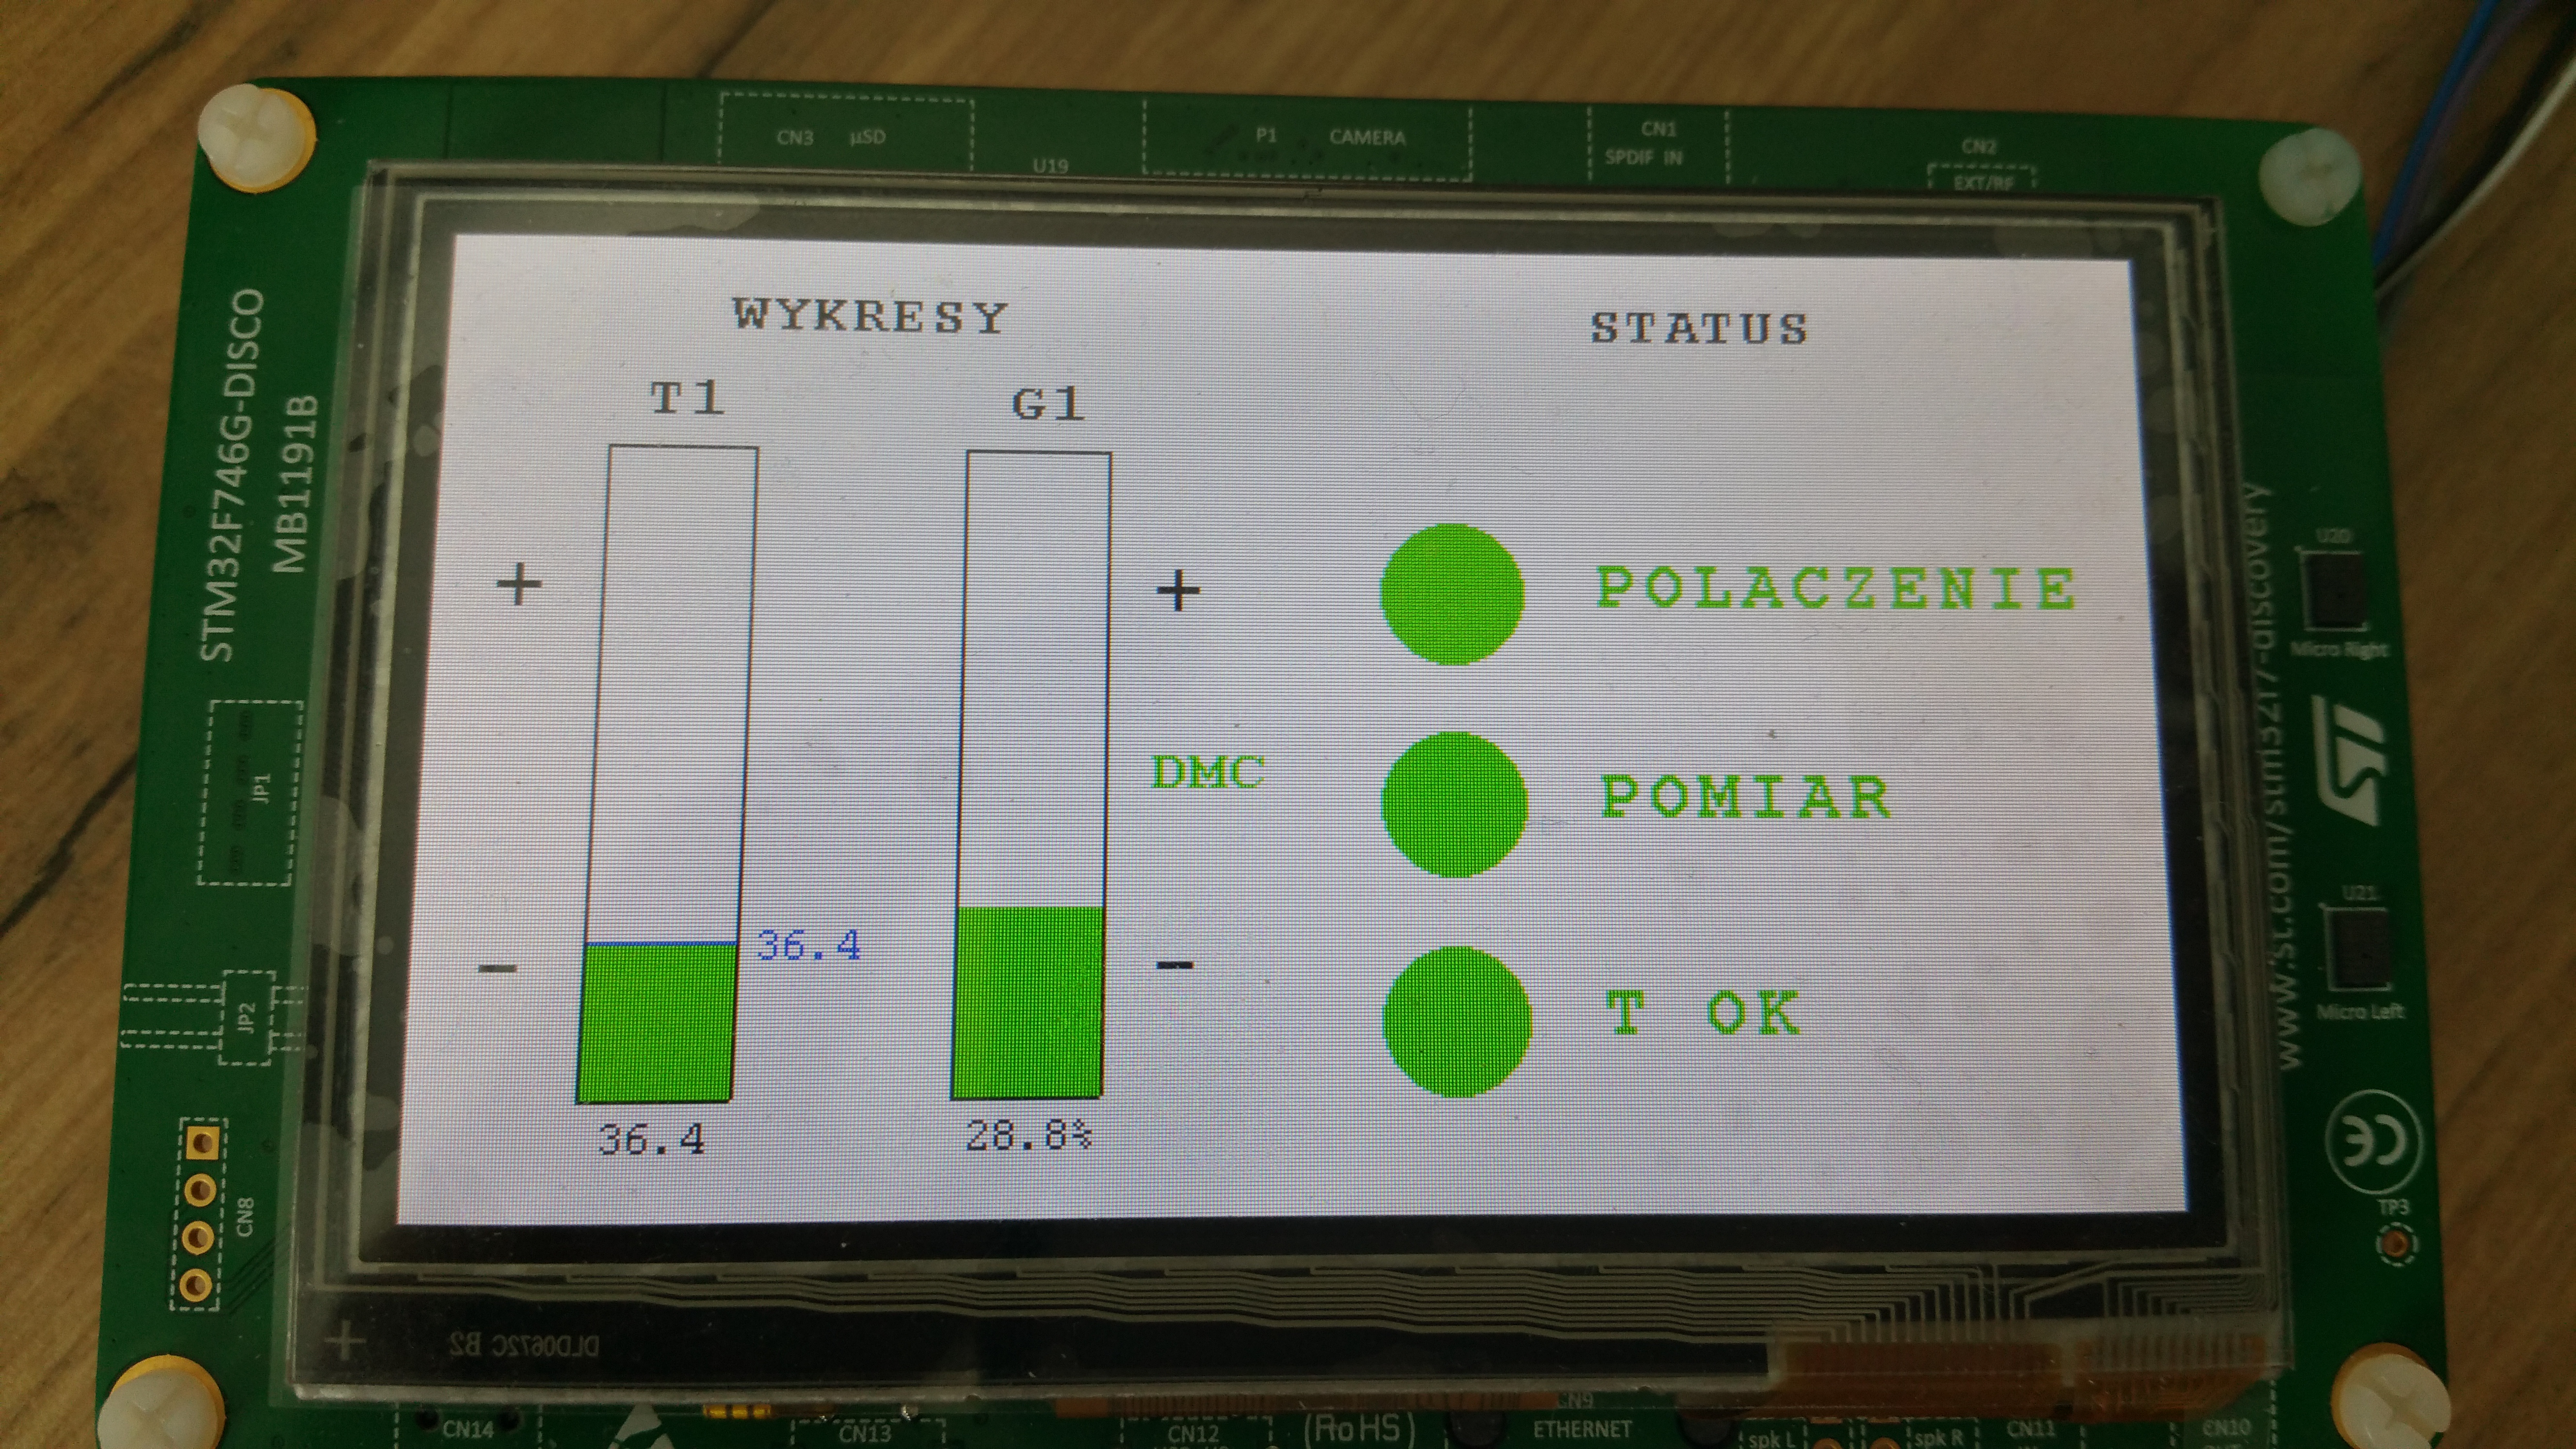
\includegraphics[width=\textwidth]{im/4.jpg}
\label{R4}
\end{figure}


Jako sytuację alarmową przyjęto sytuację, w której temperatura T1 znajdzie się poza zakresem od 30 do 50 stopni Celsjusza. Poniżej zaprezentowano wystąpienie takiej sytuacji po ustawieniu temperatury zadanej powyżej tego zakresu. Jest ona wyraźnie sygnalizowana w polu statusu poprzez zmianę ``lampki'' temperatury oraz jej opisu. Gdy temperatura jest za wysoka kolor zmienia się na czerwony, a napis na ``T WYSOKA'', a gdy spadnie poniżej 30 stopni, kolor zmieni się na niebieski, a napis na ``T NISKA''.


\begin{figure}[H]
\centering
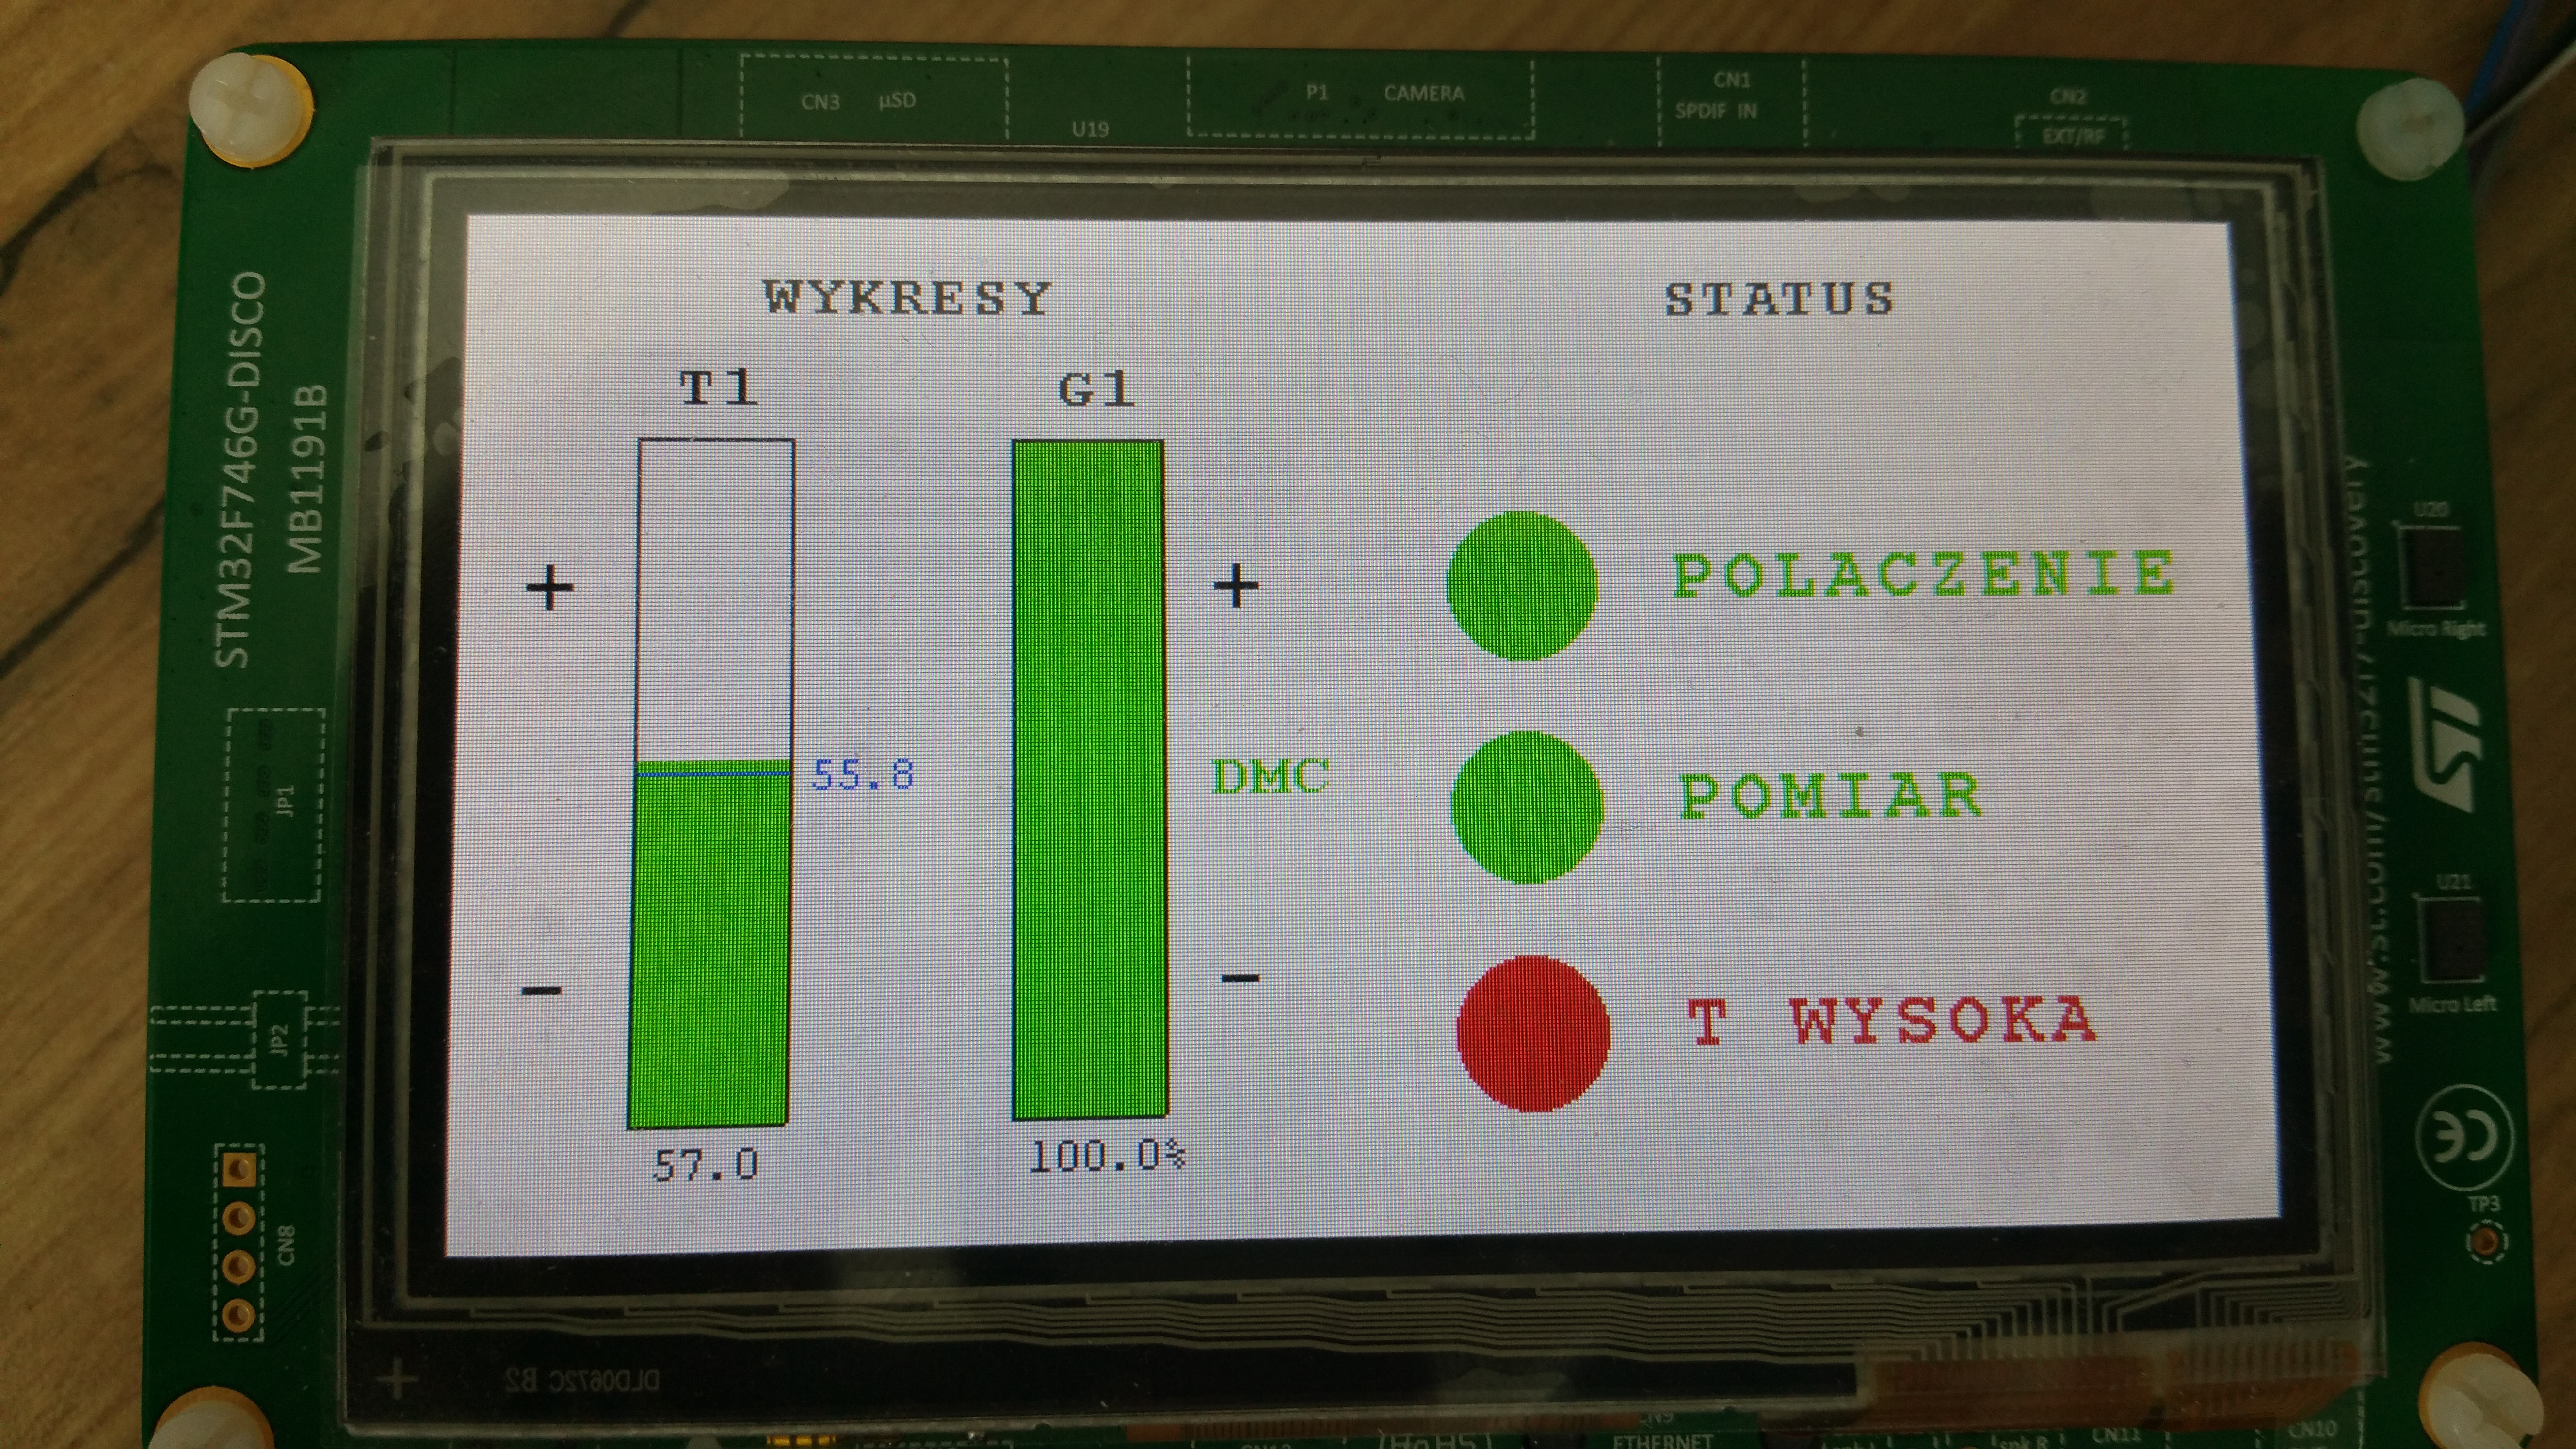
\includegraphics[width=\textwidth]{im/1.jpg}
\label{R1}
\end{figure}


Podobnie sygnalizowane jest wystąpienie błędu pomiaru.


\begin{figure}[H]
\centering
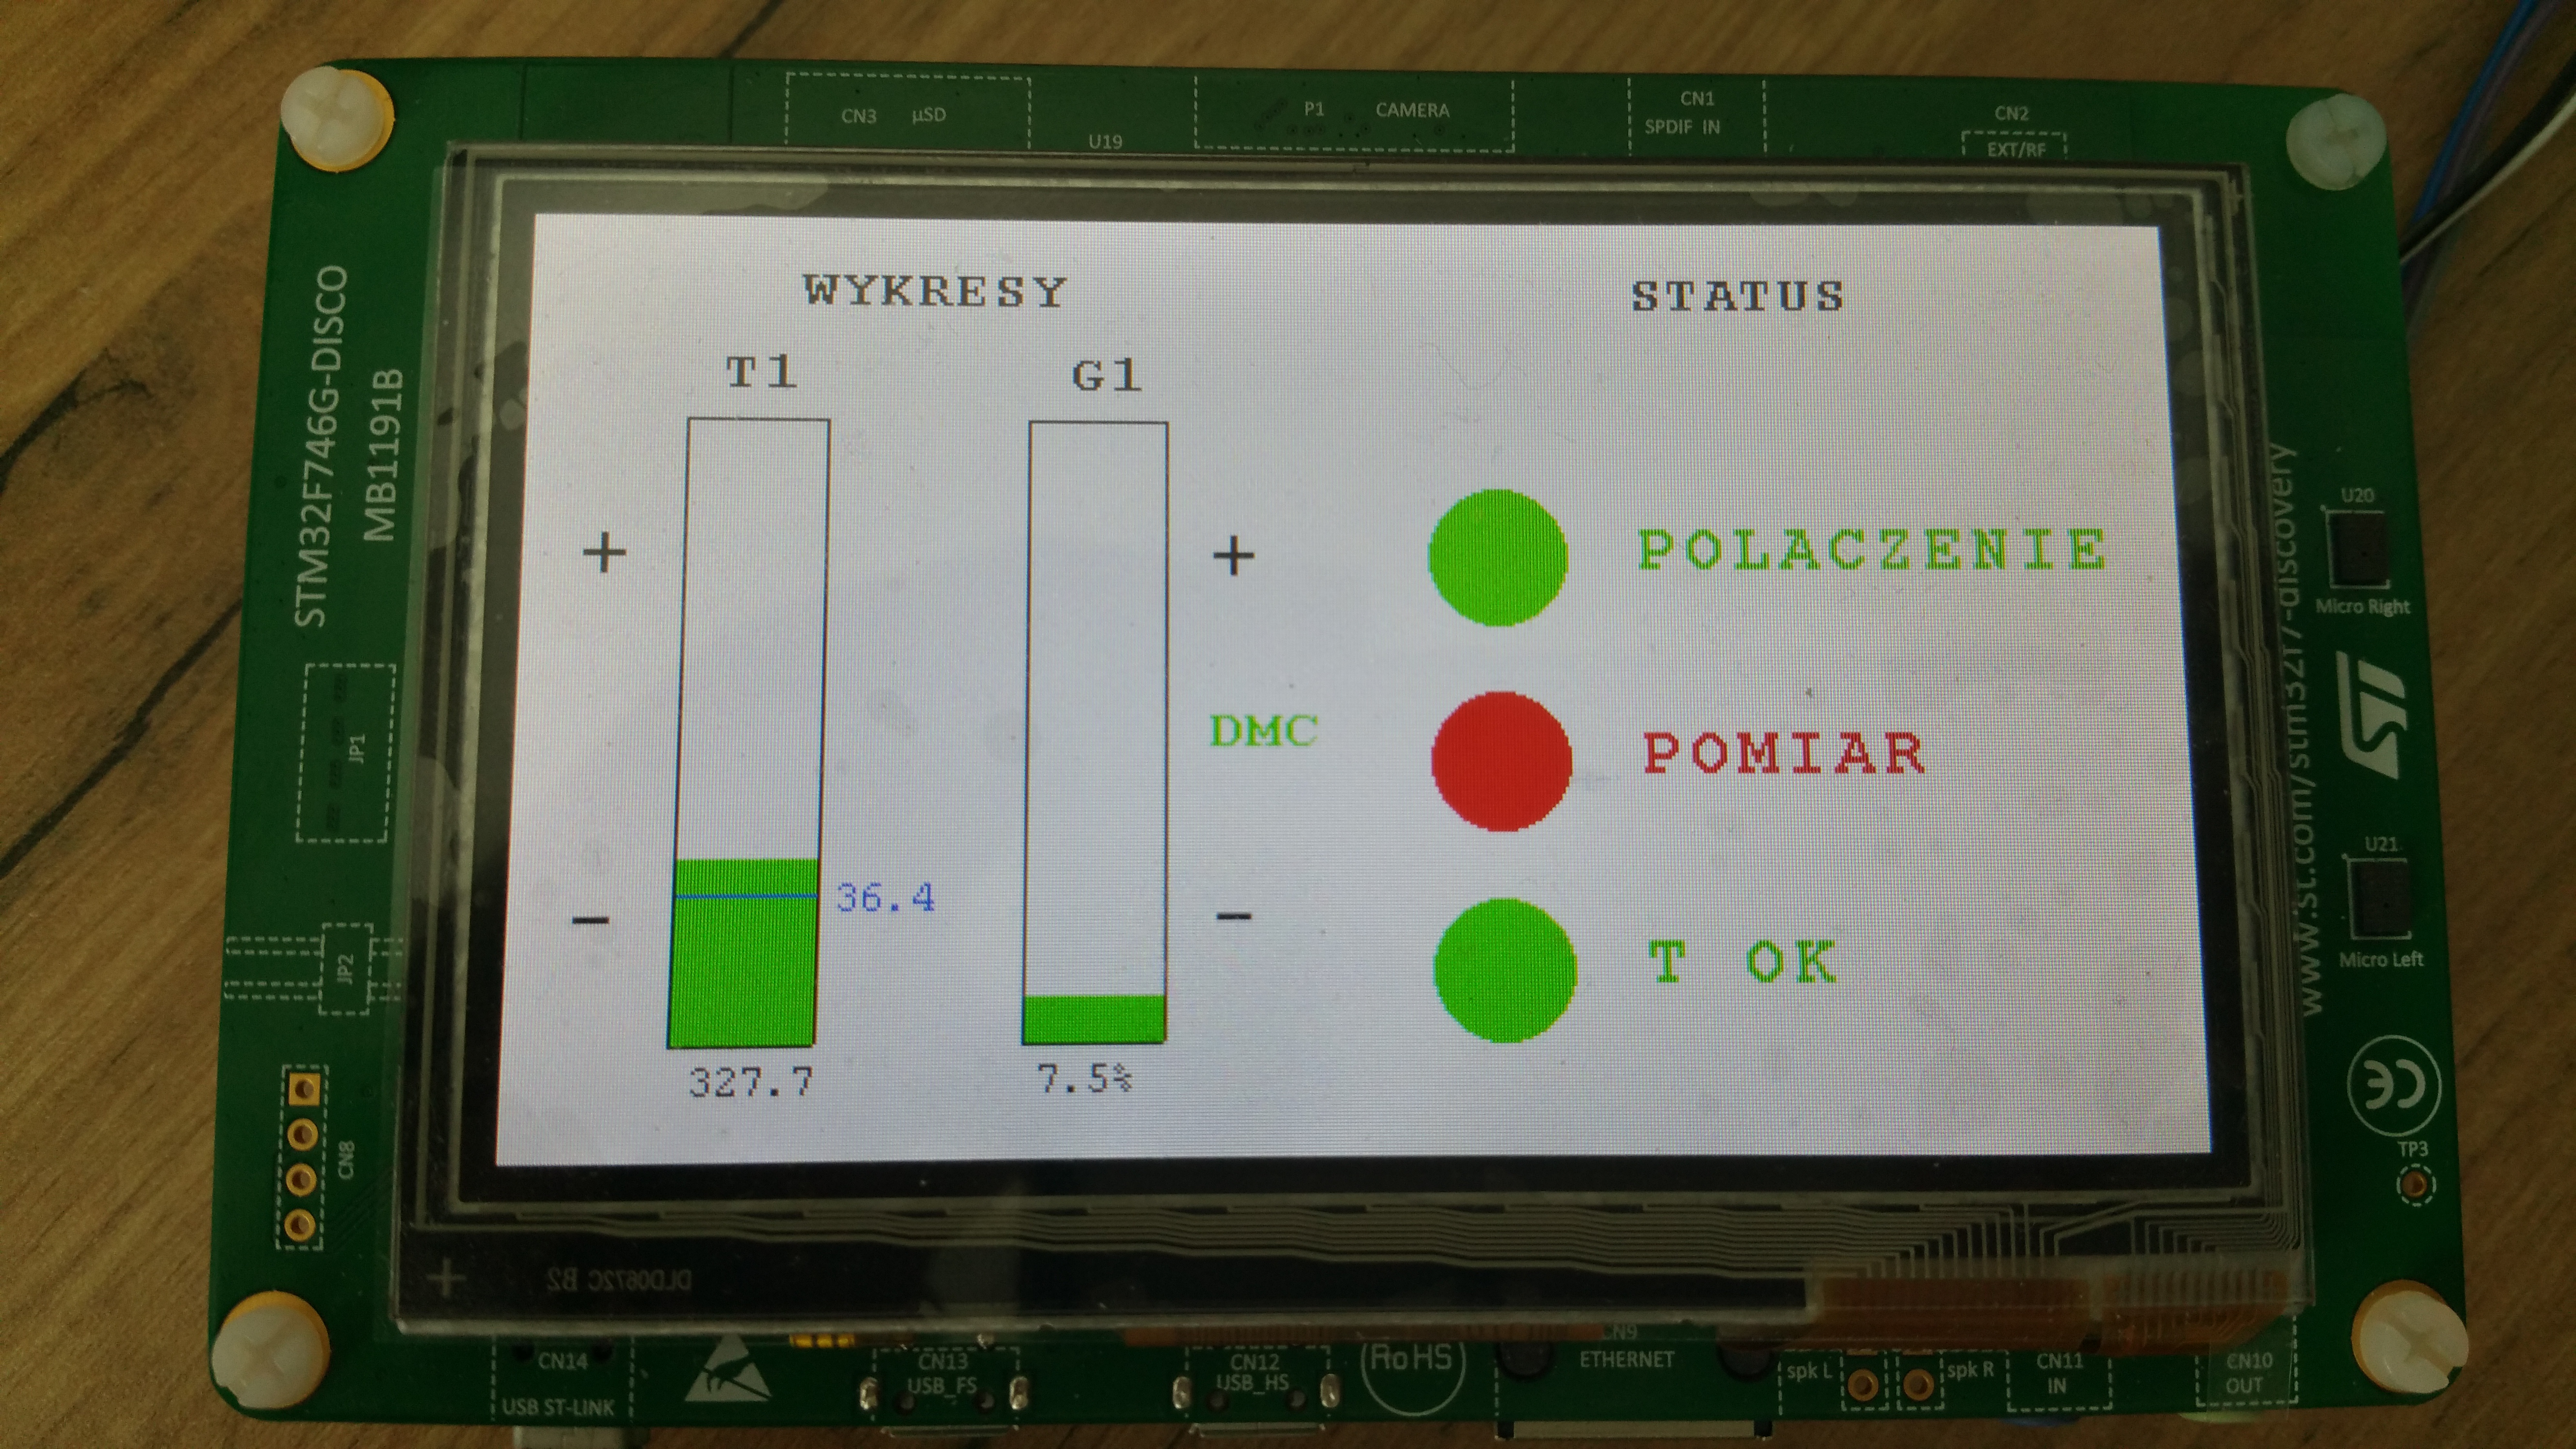
\includegraphics[width=\textwidth]{im/3.jpg}
\label{R3}
\end{figure}


Układ operuje w dwóch trybach: DMC i manualnym, przejście między trybami odbywa się poprzez dotknięcie napisu sygnalizującego obecny stan, wyświetla on odpowiednio napisy ``DMC'' i ``MAN''. W trybie manualnym wciskanie plusa i minusa na prawo od słupka G1 powoduje zmianę wartości sterowania grzałki.


\begin{figure}[H]
\centering
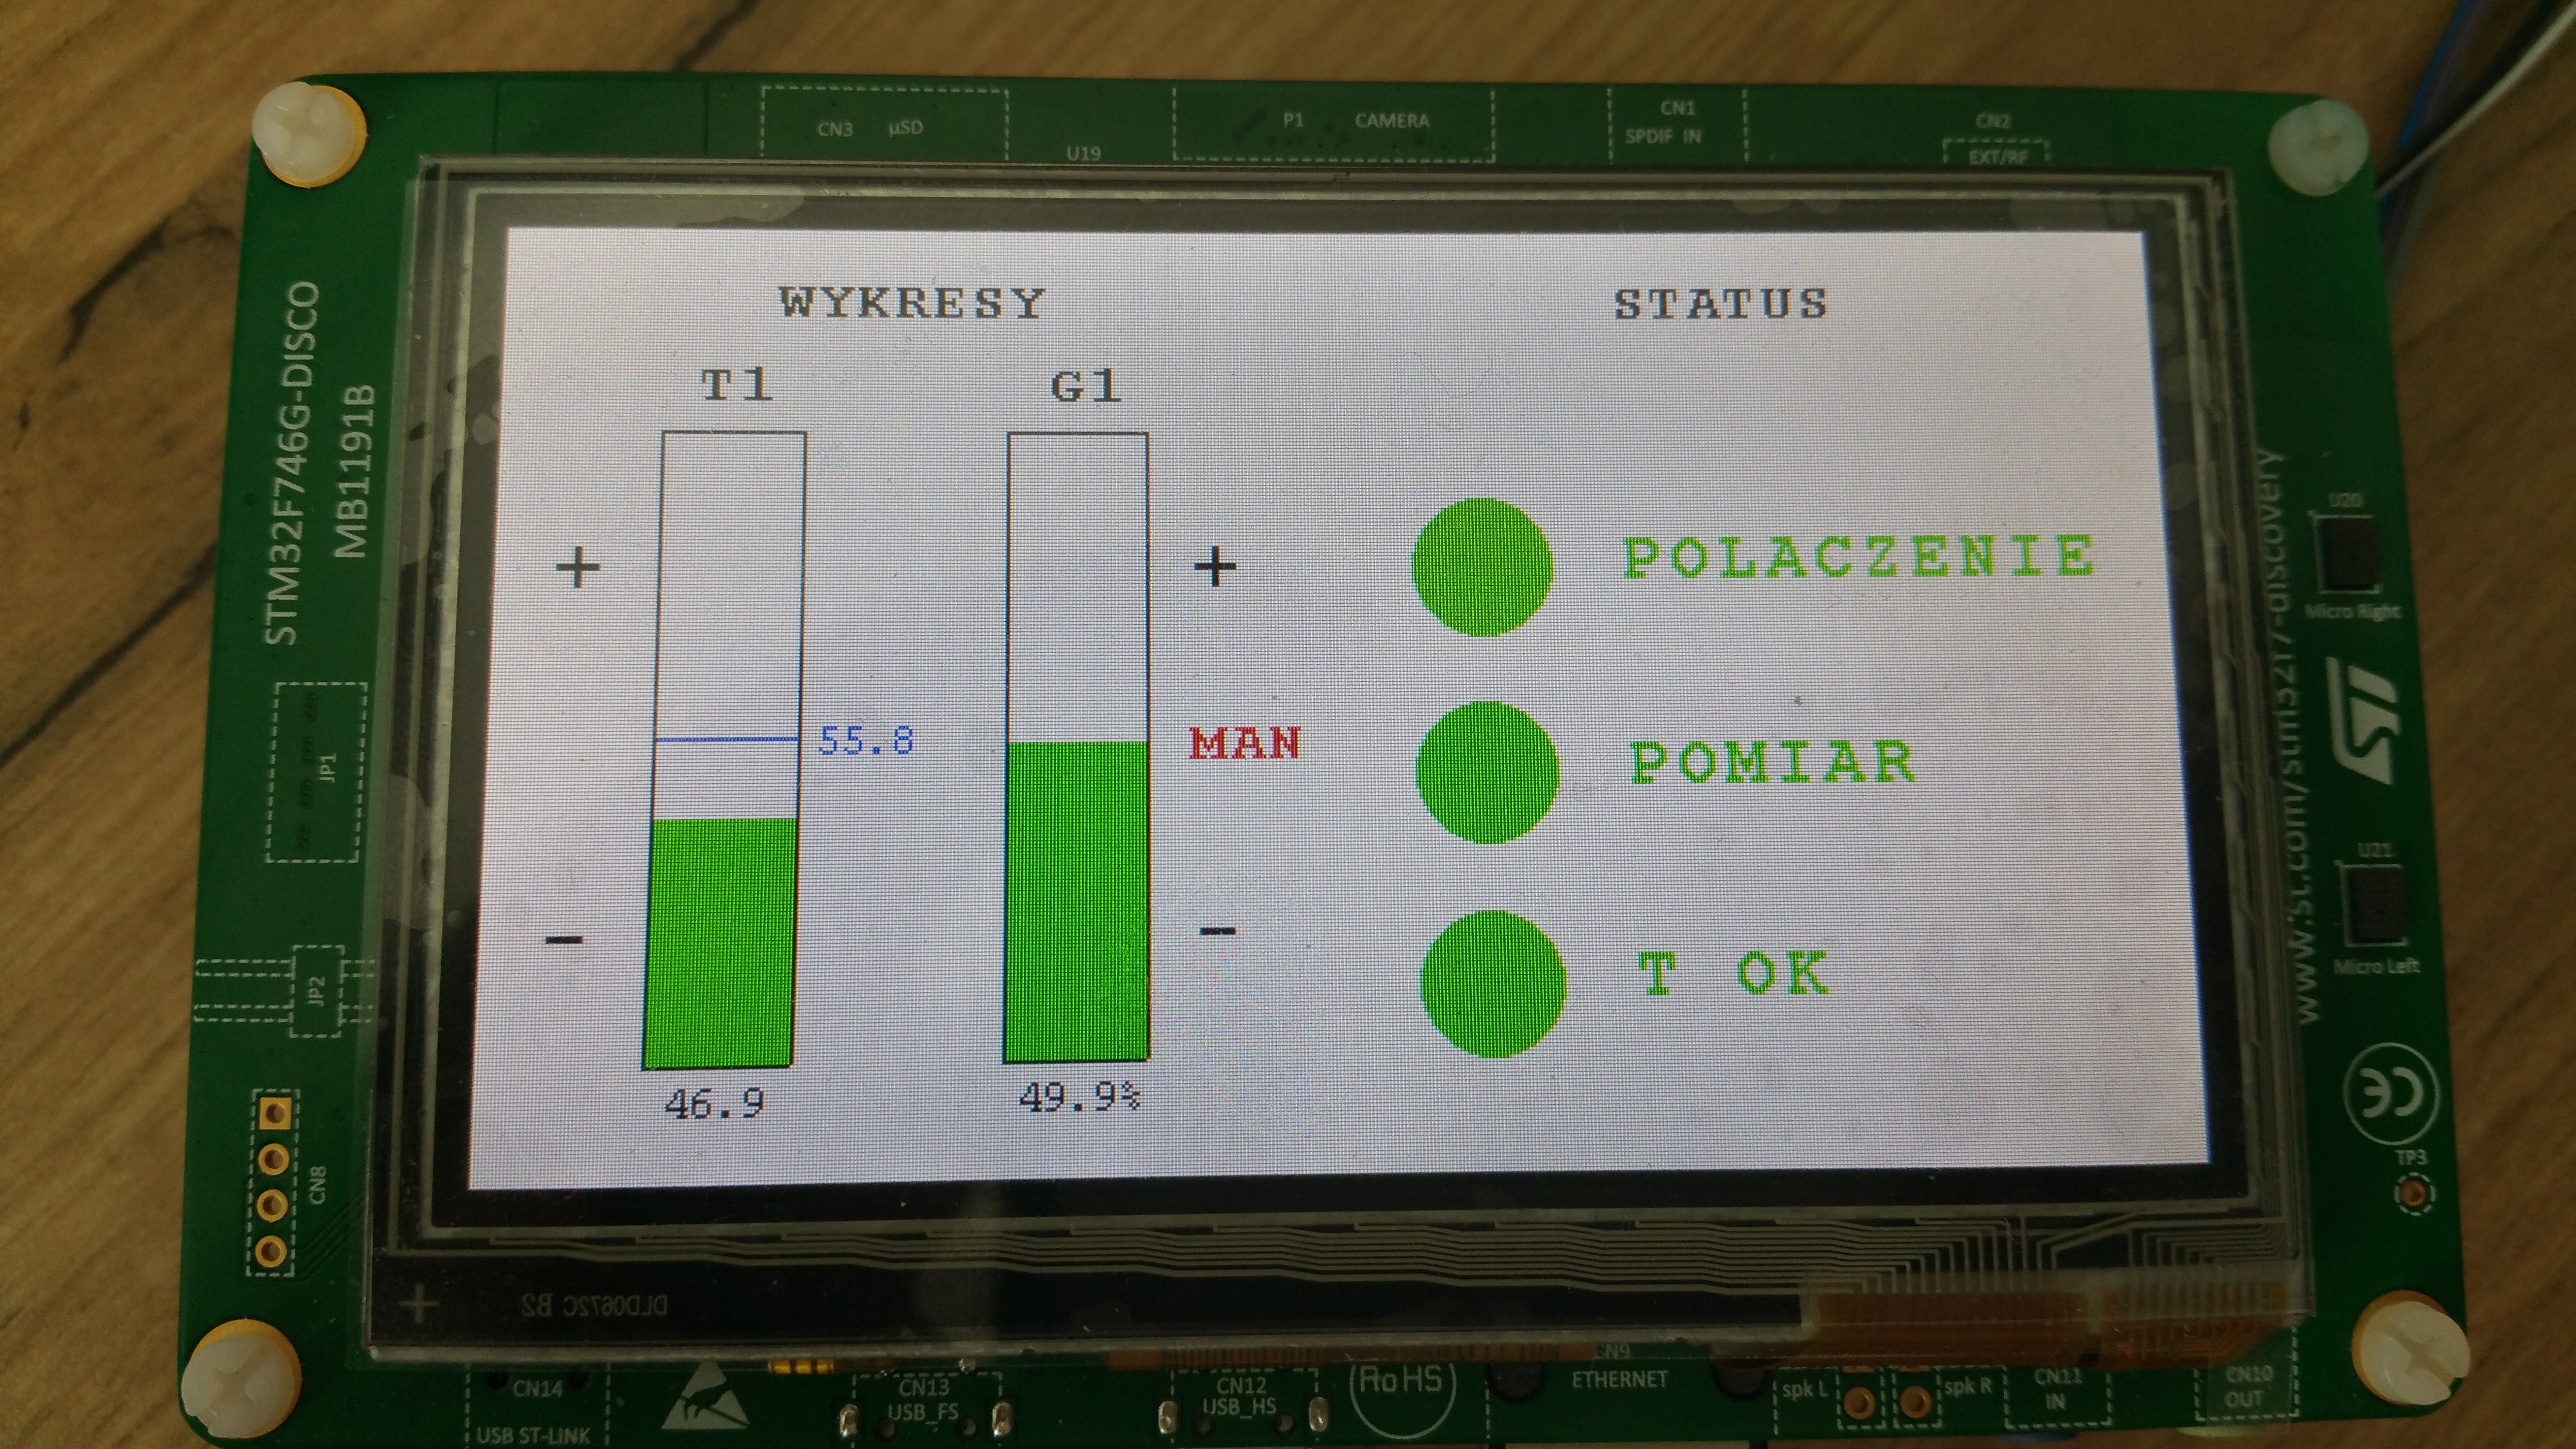
\includegraphics[width=\textwidth]{im/2.jpg}
\label{R2}
\end{figure}


Ponieważ wystąpienie błędu w komunikacji sygnalizuje poważny problem --- zgodnie z zaleceniem --- sygnalizujemy go poprzez wyświetlenie dużego napisu na czerwonym tle. Jeżeli problem zniknie samoczynnie to dla informacji operatora układ wyświetla wszystkie dane na czerwonym tle i informuje napisem o wystąpieniu błędu, aż do zrestartowania przez niego całego systemu.


\begin{figure}[H]
\centering
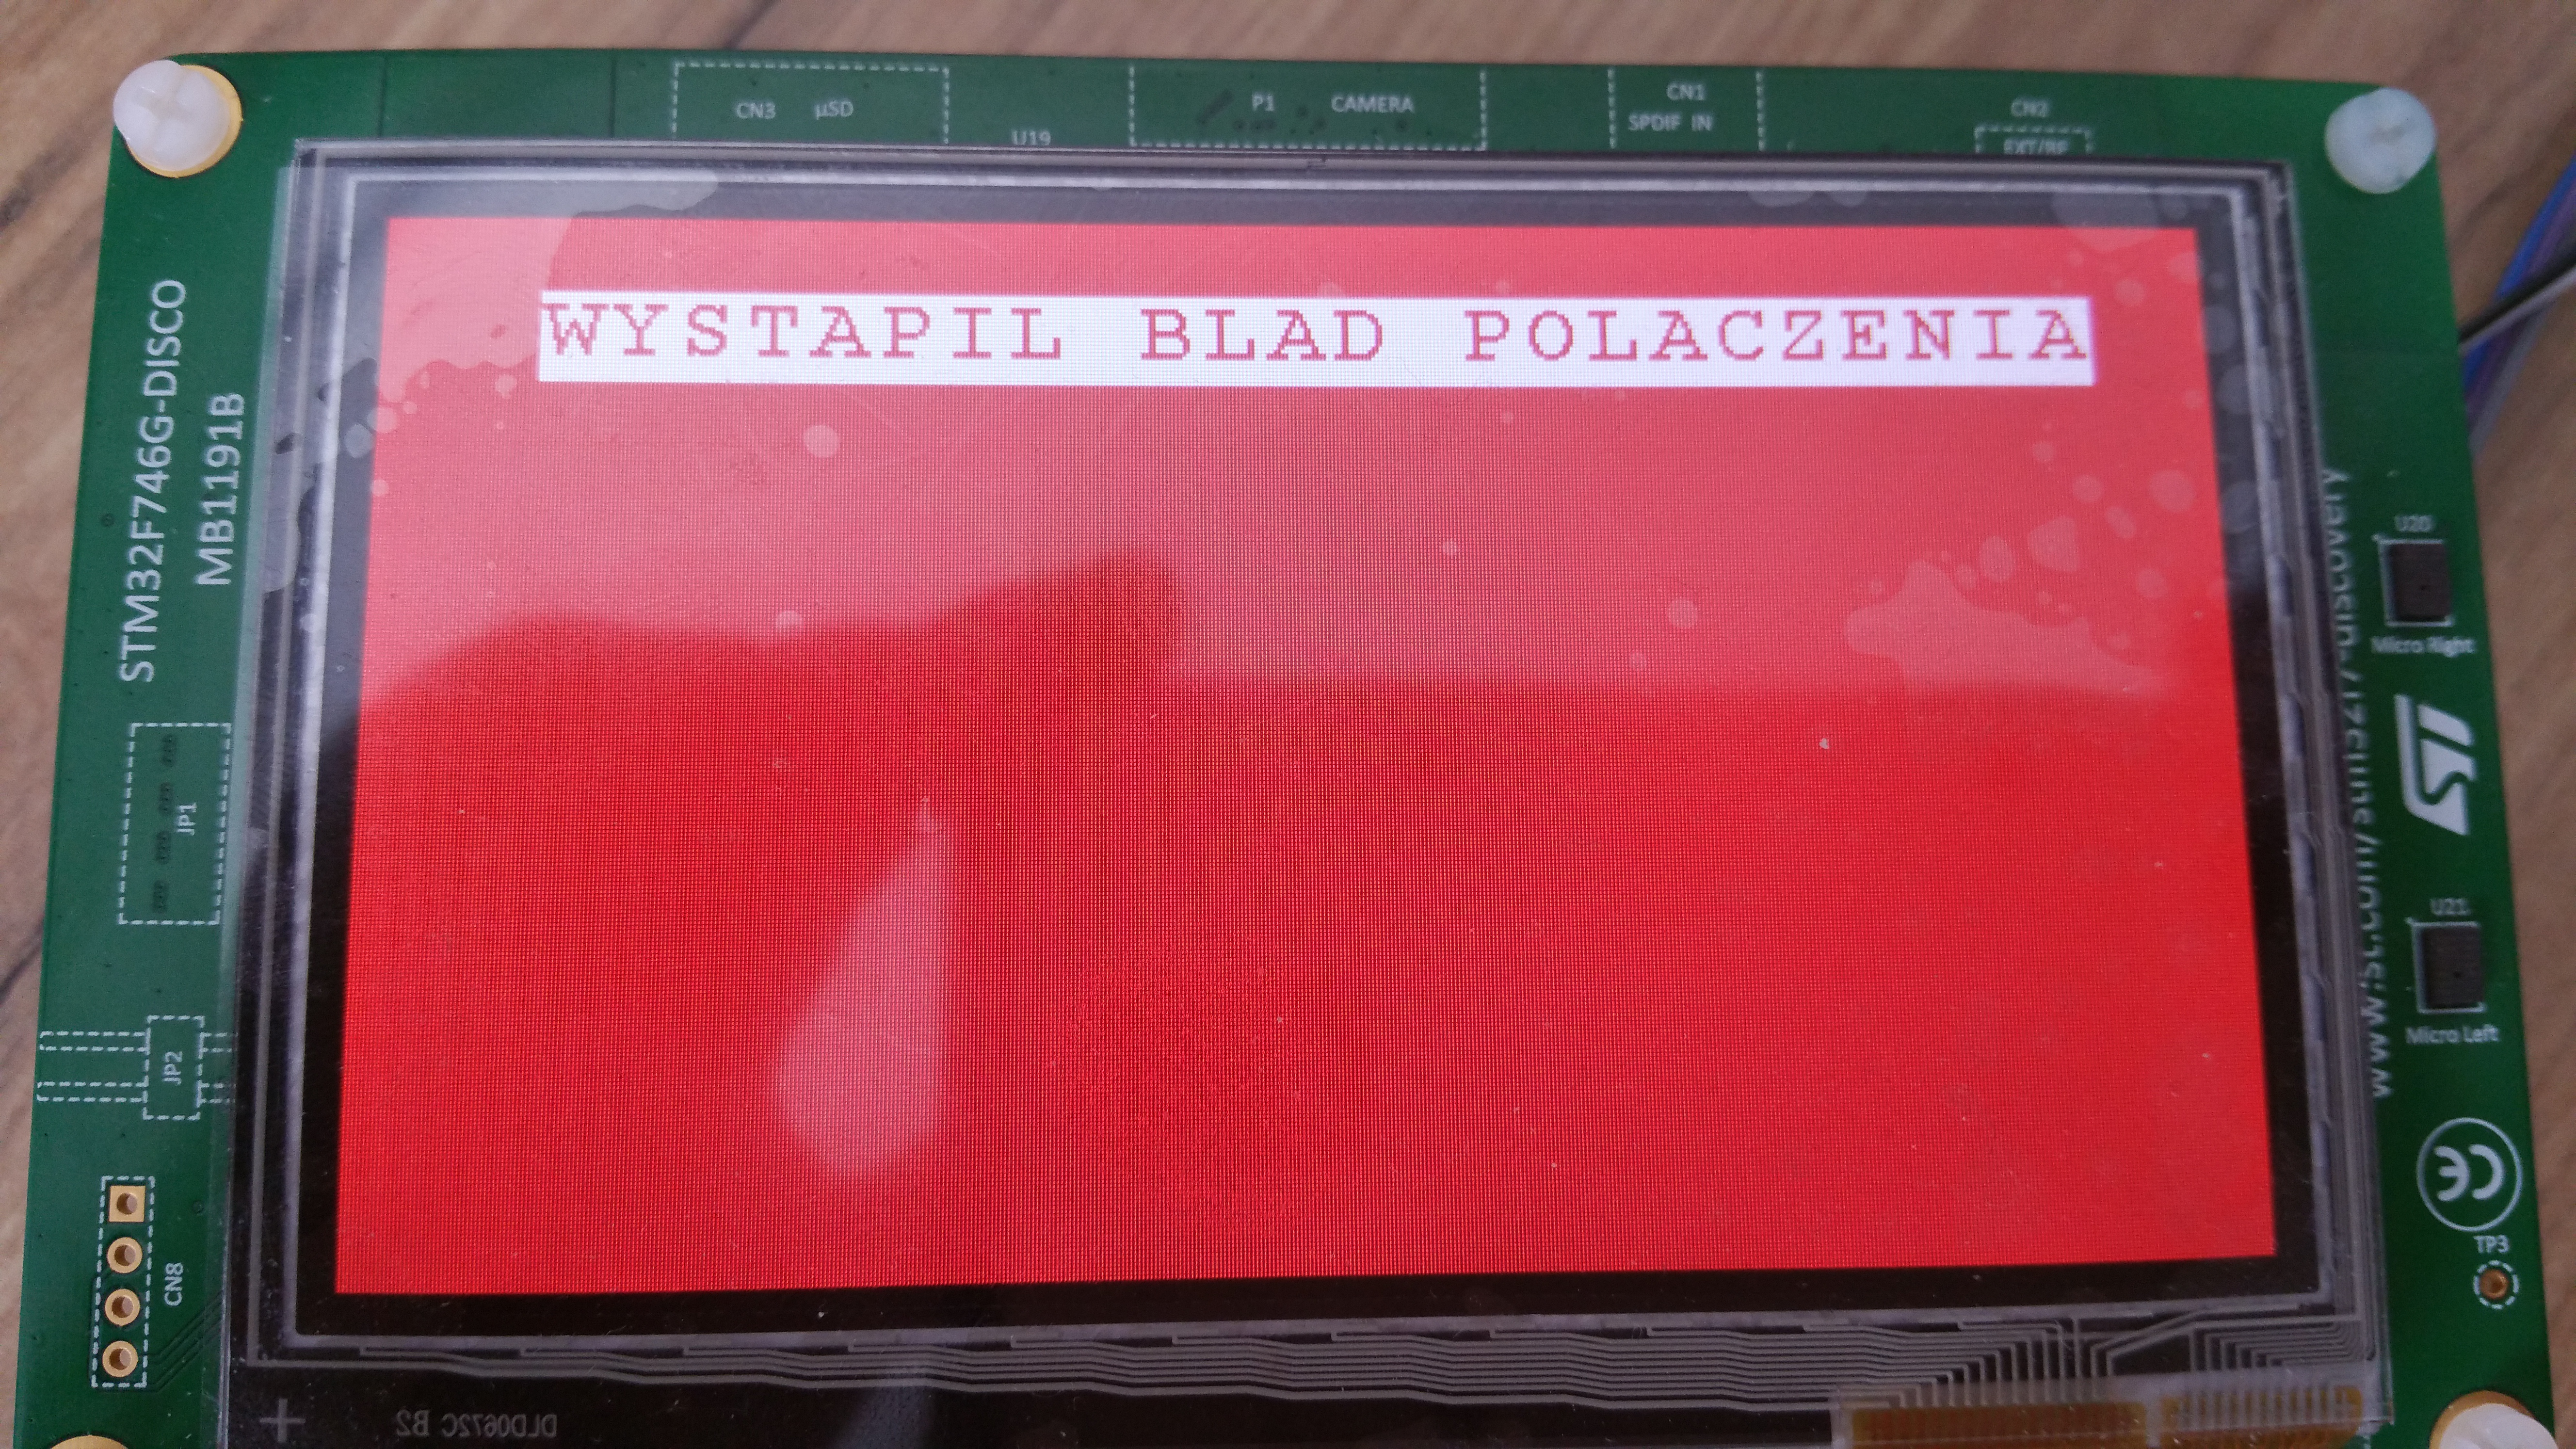
\includegraphics[width=\textwidth]{im/5.jpg}
\label{R5}
\end{figure}


\begin{figure}[H]
\centering
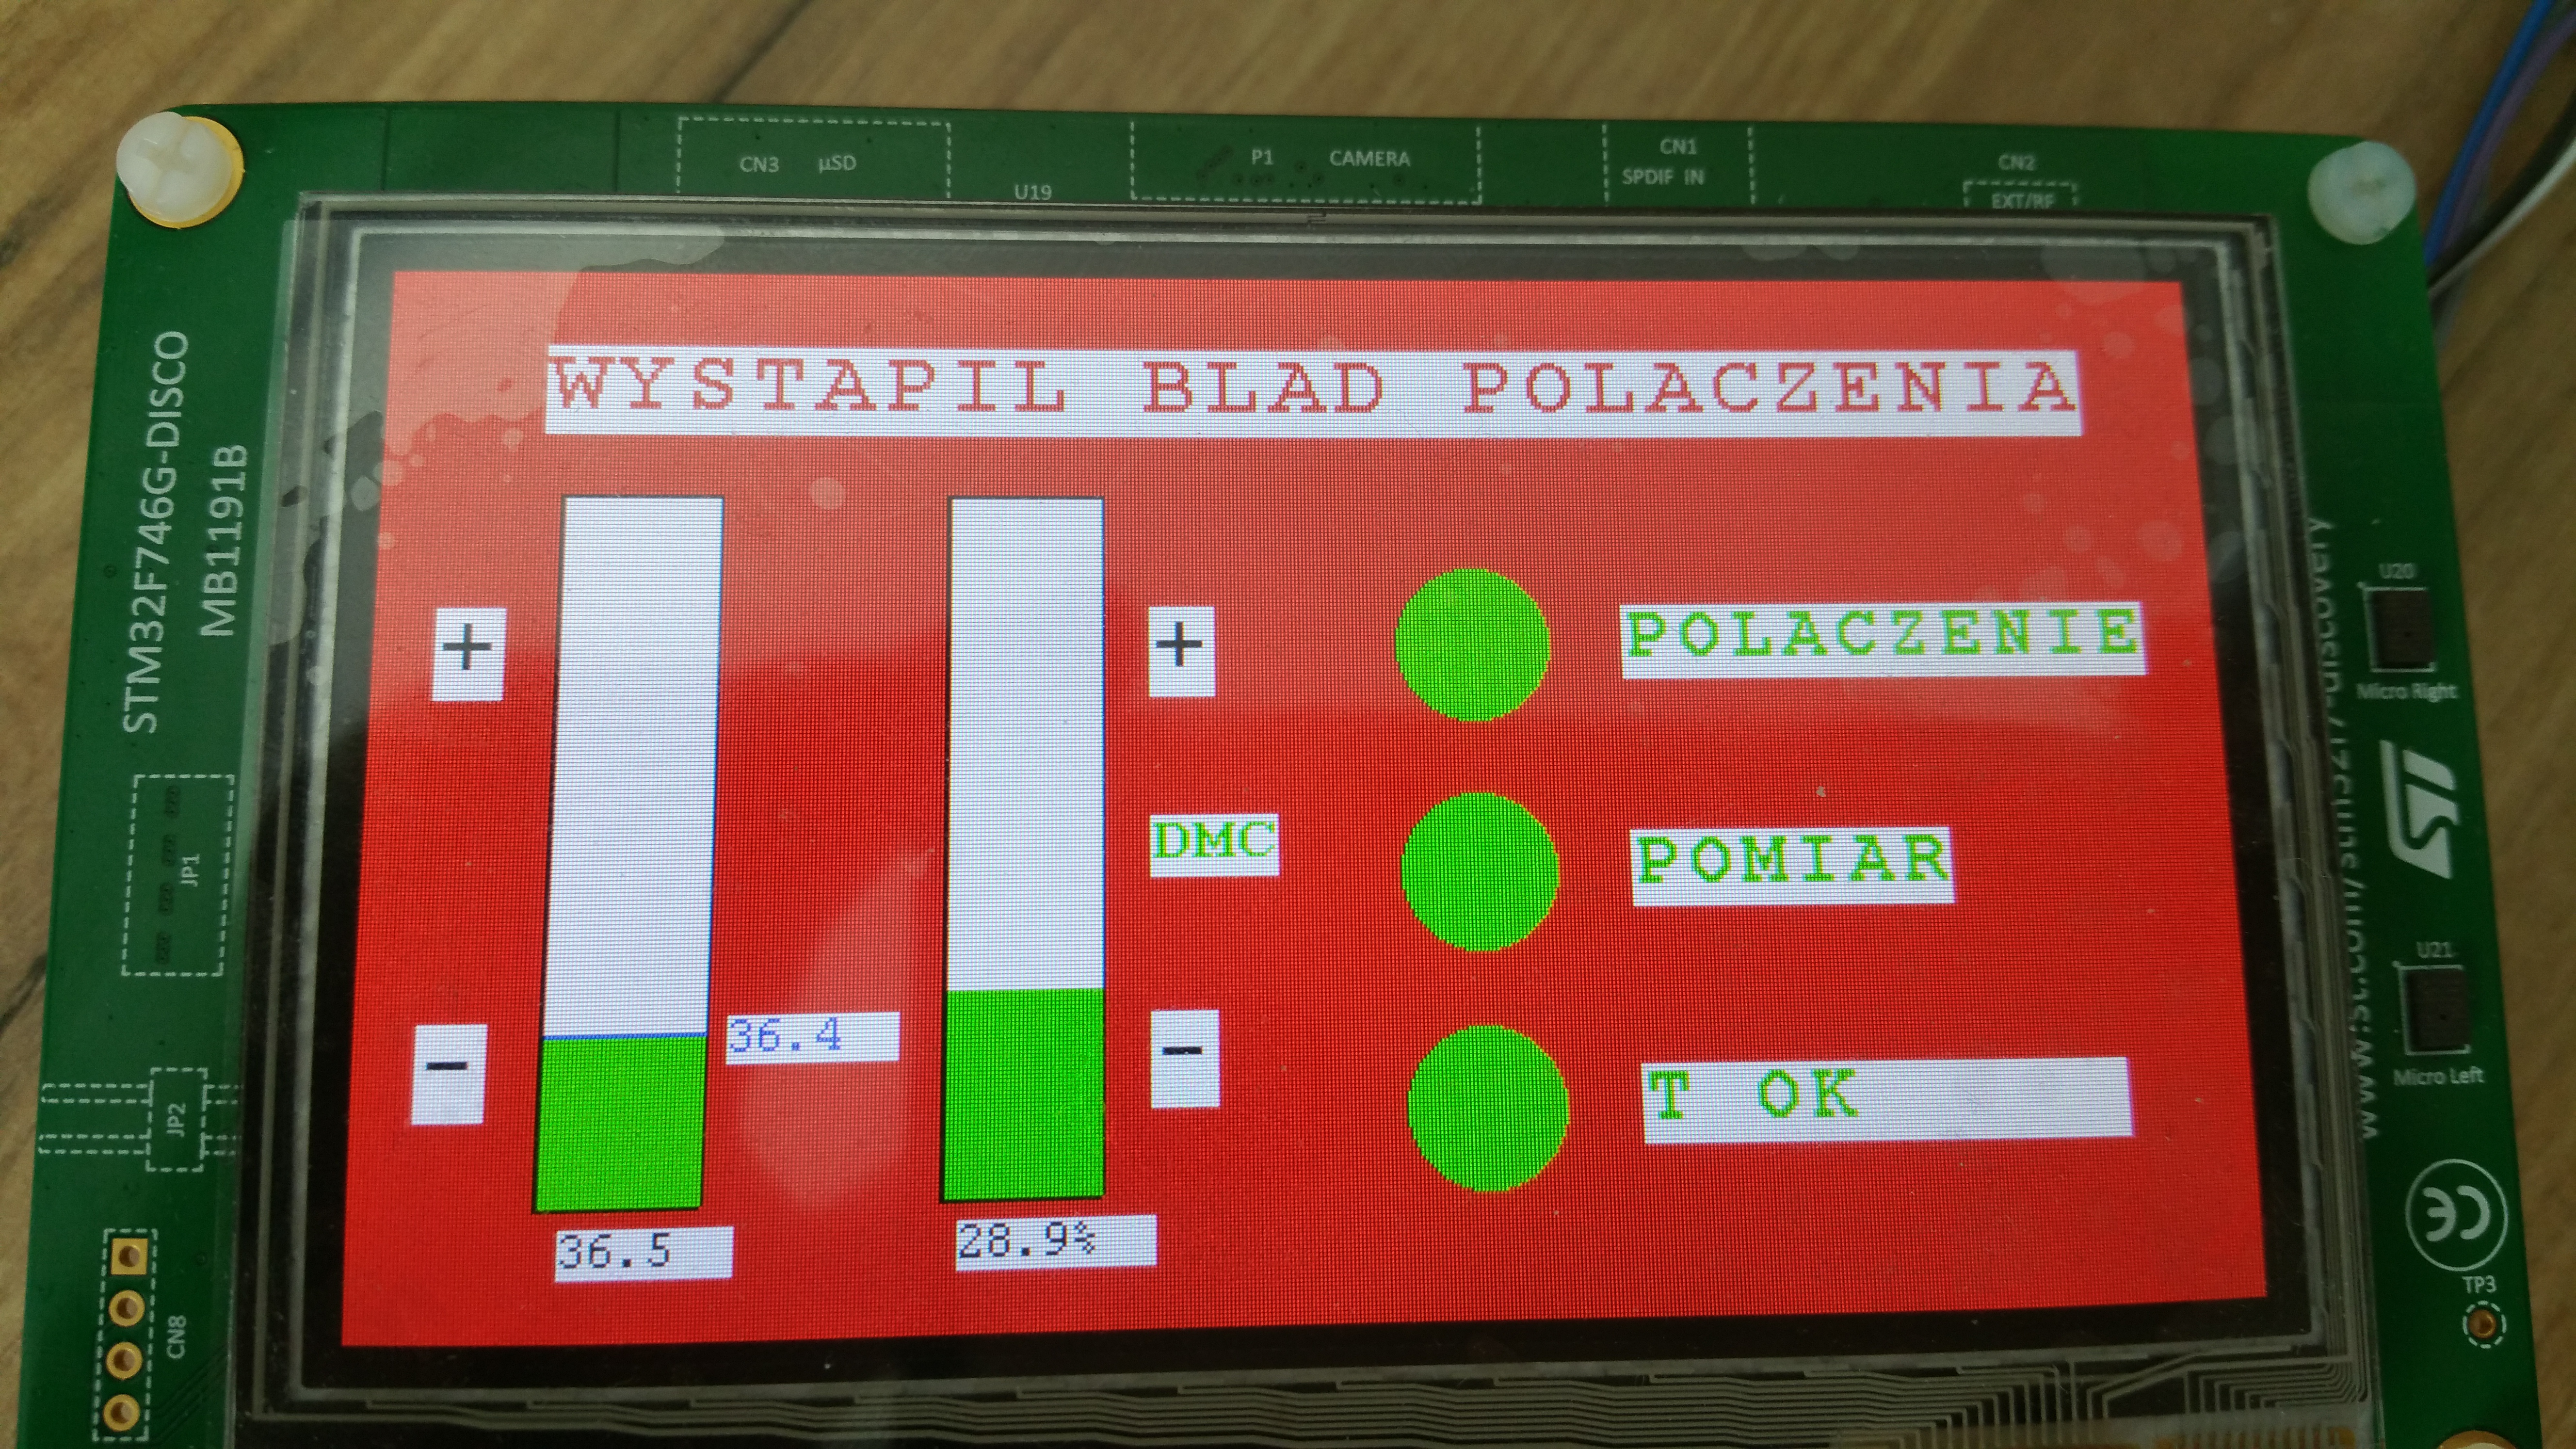
\includegraphics[width=\textwidth]{im/6.jpg}
\label{R6}
\end{figure}

